% \VignetteEngine{knitr::knitr}
\documentclass{bmcart}\usepackage[]{graphicx}\usepackage[]{color}
%% maxwidth is the original width if it is less than linewidth
%% otherwise use linewidth (to make sure the graphics do not exceed the margin)
\makeatletter
\def\maxwidth{ %
  \ifdim\Gin@nat@width>\linewidth
    \linewidth
  \else
    \Gin@nat@width
  \fi
}
\makeatother

\definecolor{fgcolor}{rgb}{0.345, 0.345, 0.345}
\newcommand{\hlnum}[1]{\textcolor[rgb]{0.686,0.059,0.569}{#1}}%
\newcommand{\hlstr}[1]{\textcolor[rgb]{0.192,0.494,0.8}{#1}}%
\newcommand{\hlcom}[1]{\textcolor[rgb]{0.678,0.584,0.686}{\textit{#1}}}%
\newcommand{\hlopt}[1]{\textcolor[rgb]{0,0,0}{#1}}%
\newcommand{\hlstd}[1]{\textcolor[rgb]{0.345,0.345,0.345}{#1}}%
\newcommand{\hlkwa}[1]{\textcolor[rgb]{0.161,0.373,0.58}{\textbf{#1}}}%
\newcommand{\hlkwb}[1]{\textcolor[rgb]{0.69,0.353,0.396}{#1}}%
\newcommand{\hlkwc}[1]{\textcolor[rgb]{0.333,0.667,0.333}{#1}}%
\newcommand{\hlkwd}[1]{\textcolor[rgb]{0.737,0.353,0.396}{\textbf{#1}}}%

\usepackage{framed}
\makeatletter
\newenvironment{kframe}{%
 \def\at@end@of@kframe{}%
 \ifinner\ifhmode%
  \def\at@end@of@kframe{\end{minipage}}%
  \begin{minipage}{\columnwidth}%
 \fi\fi%
 \def\FrameCommand##1{\hskip\@totalleftmargin \hskip-\fboxsep
 \colorbox{shadecolor}{##1}\hskip-\fboxsep
     % There is no \\@totalrightmargin, so:
     \hskip-\linewidth \hskip-\@totalleftmargin \hskip\columnwidth}%
 \MakeFramed {\advance\hsize-\width
   \@totalleftmargin\z@ \linewidth\hsize
   \@setminipage}}%
 {\par\unskip\endMakeFramed%
 \at@end@of@kframe}
\makeatother

\definecolor{shadecolor}{rgb}{.97, .97, .97}
\definecolor{messagecolor}{rgb}{0, 0, 0}
\definecolor{warningcolor}{rgb}{1, 0, 1}
\definecolor{errorcolor}{rgb}{1, 0, 0}
\newenvironment{knitrout}{}{} % an empty environment to be redefined in TeX

\usepackage{alltt}

\usepackage{xcolor}
\usepackage{url}
\usepackage{amsmath}
\usepackage{amsthm}
\usepackage{amssymb}
\usepackage{graphicx}
\usepackage{tikz}
\usetikzlibrary{shapes,arrows}
\usepackage{float}
\usepackage{verbatim}
\usepackage{tabu}
\usepackage{multirow}

% \usepackage{hyperref}
% \hypersetup{
%      colorlinks   = true,
%      citecolor    = black
% }
% \hypersetup{linkcolor=black}
% \hypersetup{linkcolor=black}
% \hypersetup{linkcolor=black}

\newcommand{\beginsupplement}{%
        \setcounter{table}{0}
        \renewcommand{\thetable}{S\arabic{table}}%
        \setcounter{figure}{0}
        \renewcommand{\thefigure}{S\arabic{figure}}%
     }

% \usepackage{authblk}
\usepackage[utf8]{inputenc} %unicode support

\newcommand{\sig}{\sigma^{70}}
\IfFileExists{upquote.sty}{\usepackage{upquote}}{}
\begin{document}

\begin{frontmatter}

\begin{fmbox}
\dochead{Draft}

\title{Data exploration, quality control and statistical analysis of
  ChIP-exo experiments}

\author[
   addressref={aff1},
   noteref={n1},
   email={welch@stat.wisc.edu}      
]{\inits{RW}\fnm{Rene} \snm{Welch} }
\author[
   addressref={aff6},        % id's of addresses, e.g. {aff1,aff2}
   noteref={n1},
   email={chungd@musc.edu}   % email address
]{\inits{DC}\fnm{Dongjun} \snm{Chung} } 
\author[
   addressref={aff3},
   email={ong@cs.wisc.edu}
]{\inits{IO}\fnm{Irene} \snm{Ong}}
\author[
   addressref={aff3,aff4},
   email={jagrass@wisc.edu}
]{\inits{JG}\fnm{Jeffrey} \snm{Grass}}
\author[
   addressref={aff3,aff4,aff5},
   email={landick@bact.wisc.edu}
]{\inits{RL}\fnm{Robert} \snm{Landick}}
\author[
   addressref={aff1,aff2},
   corref={aff1},
   email={keles@stat.wisc.edu}
]{\inits{SK}\fnm{S\"und\"uz} \snm{Kele\c{s}}}

\address[id=aff1]{%                           % unique id
  \orgname{Department of Statistics, University of Wisconsin Madison}, % university, etc
  \street{1300 University Avenue},                     %
  %\postcode{}                                % post or zip code
  \city{Madison},                              % city
  \cny{WI}                                    % country
}

\address[id=aff2]{%
  \orgname{Department of Biostatistics and Medical Informatics, University of Wisconsin Madison},
  \street{600 Highland Avenue},
%  \postcode{24105}
  \city{Madison},
  \cny{WI}
}
\address[id=aff3]{
  \orgname{Great Lakes Bioenergy Research Center, University of Wisconsin Madison},
  \street{1552 University Avenue},
  \city{Madison},
  \cny{WI}
}
\address[id=aff4]{
  \orgname{Department of Biochemistry, University of Wisconsin Madison},
  \street{433 Babcock Drive},
  \city{Madison},
  \cny{WI}
}
\address[id=aff5]{
  \orgname{Department of Bacteriology, University of Wisconsin Madison},
  \street{1550 Linden Drive},
  \city{Madison},
  \cny{WI}
}
\address[id=aff6]{
  \orgname{Department of Public Health Sciences, Medical University of South Carolina},
  \street{135 Cannon Street},
  \city{Charleston},
  \cny{SC}
}


\begin{artnotes}
\note[id=n1]{These two authors contributed equally.} % note, connected to author
\end{artnotes}


\end{fmbox}

\begin{abstractbox}

  \begin{abstract}

    ChIP-exo is a modification of the ChIP-Seq protocol for high
    resolution mapping of transcription factor binding sites. Although
    many aspects of the ChIP-exo data analysis are similar to those of
    ChIP-Seq, ChIP-exo presents a number of unique challenges. We
    present a quality control pipeline to evaluate a number of key
    issues including strand imbalance, library complexity and
    enrichment. Assessment of these characteristics are facilitated
    through diagnostic plots and summary statistics calculated over
    regions of the genome with varying levels of coverage.

    The pipeline explores and quantifies these aspects by partitioning
    the experiment reads into a collection of regions, calculating a
    series of summary statistics for each region, providing
    visualizations and calculating measures to globally asses the
    quality of a ChIP-exo experiment. We provide guidelines to
    distinguish libraries with low complexity from deeply sequenced
    experiments by the use of the QC pipeline. We demonstrate that the
    ChIP-exo QC pipeline it is also applicable to ChIP-nexus data,
    showing that those experiments present higher quality than
    ChIP-exo experiments under similar conditions.

    We compared ChIP-exo with Paired End (PE) and Single End (SE)
    ChIP-Seq and found the following characteristics: First, although
    often assumed in ChIP-exo data analysis methods, the ``peak pair''
    assumptions does not hold locally in actual ChIP-exo data. Second,
    we for the first time compared PE ChIP-Seq with ChIP-exo and found
    that at fixed sequencing depths, ChIP-exo provides higher
    sensitivity, specificity and spatial resolution than PE
    ChIP-Seq. Finally, we show that ChIP-exo and PE ChIP-Seq are
    comparable in sensitivity for closely located binding events, but
    as the average distance between binding events increases, ChIP-exo
    show higher sensitivity than PE ChIP-Seq.

    % both protocols are comparable in resolutions and sensitivity for
    % closely located binding events, but as the distance between
    % binding events increases ChIP-exo shows higher sensitivity that
    % PE ChIP-Seq. Finally, at fixed sequencing depths, ChIP-exo
    % provides higher sensitivity, specificity and spatial resolution
    % than PE ChIP-Seq.
  \end{abstract}

\begin{keyword}
  \kwd{ChIP-exo}
  \kwd{ChIP-nexus}
  \kwd{ChIP-Seq}
  \kwd{Quality Control}
  \kwd{Spatial Resolution}
  \kwd{Transcription Factor}  
  \kwd{Binding Site Identification on High-Res}
  \kwd{Deconvolution}
\end{keyword}

\end{abstractbox}

\end{frontmatter}

\newpage

\section*{Background}
\label{sec:intro}

ChIP-exo (Chromatin Immunoprecipitation followed by exonuclease
digestion and next generation sequencing) Rhee and Pugh, 2011
\nocite{exo1} is the state-of-the-art experiment developed to attain
single base-pair resolution of protein binding site identification and
it is considered as a powerful alternative to popularly used ChIP-Seq
(Chromatin Immunoprecipitation coupled with next generation
sequencing) assay. ChIP-exo experiments first capture millions of DNA
fragments (150 - 250 bp in length) that the protein under study
interacts with using random fragmentation of DNA and a
protein-specific antibody. Then, exonuclease is introduced to trim the
$5\prime$ end of each DNA fragment to a fixed distance from the bound
protein compared to ChIP-Seq. This step is unique to ChIP-exo and
could potentially provide significantly higher spatial resolution
compared to ChIP-Seq. Finally, high throughput sequencing of a small
region (36 to 100 bp) at the $5\prime$ end of each fragment generates
millions of reads. Figure \ref{fig:chip_diagram} illustrates the
differences between ChIP-exo, Single End (SE) ChIP-Seq and Paired End
(PE) ChIP-Seq: The $5\prime$ ends of a ChIP-exo experiment are located
more tightly around the binding proteins than in a ChIP-Seq
experiment; in a PE ChIP-Seq experiment both ends are observed while
in a SE ChIP-Seq experiment only the $5\prime$ end.

ChIP-nexus (Chromatin Immunoprecipitation followed by exonuclease
digestion, unique barcode, single ligation and next generation
ligation) He et al., 2015 \nocite{chipnexus} is a modification to the
ChIP-exo protocol, where both sequencing adaptors are ligated at the
end of the ChIP fragments. Then, after exonuclease digestion, DNA
self-circularization with circLigase, and restriction enzyme cutting
between the two adaptors, the final library is ammplified. ChIP-nexus
arises as an alternative to ChIP-exo as it provides the possibility of
attaining higher resolution analysis and yields higher complexity
libraries.

% Refers to... First, DNA libraries... I think that these might be
% too much details for the introduction. How about discussing them in
% the results when we investigate the related

While the number of ChIP-exo data keeps increasing, characteristics of
ChIP-exo data are not fully investigated yet. First, DNA libraries
generated by the ChIP-exo protocol are expected to be less complex than the
libraries generated by ChIP-Seq (Mahony et al.,
2015\nocite{exo_review}). Second, although there are roughly the same
amount of reads in both strands, locally there may be more reads in
one strand than in the other. Finally, most of current ChIP-Seq
quality control (QC) guidelines (Landt et al., 2012\nocite{encode_qc})
may not be applicable on ChIP-exo, while there are not established QC
pipelines for ChIP-exo; previous ChIP-exo analyses used ChIP-Seq
samples to compare the resolution between experiments
\cite{exo1,exoillumina,exo2}. To address these challenges, we suggest
a collection of quality control visualizations to interrogate these
biases in a ChIP-exo experiment and globally asses the enrichment and
library complexity of a ChIP-exo sample and a procedure to distinguish
low complexity libraries from deeply sequenced experiments. This
aspect is unique to ChIP-exo, since the exonuclease enzyme it is
expected to digested the reads that are not bound to a transcription
factor, therefore the number of bases where a ChIP-exo fragment could
be potentially aligned is reduced. That way, in a high quality
ChIP-exo experiment is possible to observe a large amount of reads to
be aligned to unique position due to genomic signal instead of PCR
artifacts.

In order to obtain the potential benefits of ChIP-exo on protein
binding site identification, it is critical to use algorithms that
could fully utilize information available in ChIP-exo data. Rhee and
Pugh, 2011 \nocite{exo1} discussed that reads in the forward and reverse
strand might construct peak pairs around bound proteins, of which
heights were implicitly assumed to be symmetric. Based on this
rationale, they used the ``peak pair method'' that predicts the
midpoint of two modes of peak pairs as potential binding
sites. Recently developed ChIP-exo data analysis methods, such as Mace
(Wang et al, 20114\nocite{mace}), CexoR (Madrigal, 2015\nocite{cexor})
and Peakzilla (Bardet et al., 2013\nocite{peakzilla}), are also based
on this peak pair assumption. However, appropriateness of such
assumption was not fully evaluated in the literature yet. Furthermore,
it is still unknown which factors could affect protein binding site
identification using ChIP-exo data. In order to address this problem,
we investigated various aspects of ChIP-exo data by contrasting them
with their respective ChIP-Seq experiments.

Currently, research on statistical methods for ChIP-exo data is still
in its very early stage. Although many methods have been proposed to
identify protein binding sites from ChIP-Seq data (reviewed by
Wilbanks and Facciotti, 2012\nocite{evaluation} and Pepke and Wold,
2009 \nocite{computation}), such as MACS (Zhang et al.,
2008\nocite{macs}), CisGenome (Ji et al., 2008\nocite{cisgenome}) and
MOSAiCS (Kuan et al., 2009\nocite{mosaics}), these approaches might
not fully utilize potentials of ChIP-exo data for high resolution
identification of protein binding sites. Specifically these approaches
reveal protein binding sites only in lower resolution, i.e., at an
interval of hundreds to thousands of base pairs. Furthermore, they
implicitly assume that there is only one ``mode'' or ``predicted
binding location'' per this wide genomic interval. More recently,
deconvolution algorithms such as Deconvolution (Lun et al.,
2009\cite{csdeconv}), GEM (Guo et al., 2012\nocite{gem}, an improved
version of Guo et al., 2010\nocite{gps} ) and PICS (Zhang et al.,
2010\nocite{pics}) have been proposed to identify binding sites in
higher resolution using ChIP-Seq data. However, most of them are still
not tailored for ChIP-exo and PE and SE ChIP-Seq data in a unified
framework and as a result, currently available methods are not
appropriate for fair comparison between ChIP-exo and ChIP-Seq. To
address these limitations, we developed and utilized an improved
version of dPeak (Chung et al., 2013\nocite{dpeak}), a high resolution
binding site identification (deconvolution) algorithm that we
previously developed for PE and SE ChIP-Seq data, so that it can also
handle ChIP-exo data. The dPeak algorithm implements a probabilistic
model that accurately describes the ChIP-exo and ChIP-Seq data
generation process.

Some of the key findings in this work are as follows. First, we
demonstrate that the ``peak pair'' assumption of Rhee and Pugh,
2013\nocite{exo2} does not hold well in real ChIP-exo data. Second, we
found that when analyzing ChIP-exo data and the Input control is not
available, it is useful to adjust for GC content and mappability
biases to improve peak calling and binding site identification. Third,
we evaluated several methods to identify binding events and dPeak
performs competitively respect to GEM and MACE when analyzing ChIP-exo
data. Finally, when comparable number of reads is used for both
ChIP-exo and ChIP-Seq , dPeak coupled with ChIP-exo data provides
resolution comparable to PE ChIP-Seq and both significantly improve
the resolution of protein binding identification compared to SE-based
analysis with any of the available methods.

\section*{Results and discussion}
\label{sec:results}
% CTCF factor in human \cite{exo1}; ER factor in
% human and FoxA1 factor in mouse (Serandour et al., 2013
% \cite{exoillumina}); Glucocorticoid receptor (GR) in IMR90, K562 and
% U2OS cell lines (Starick et al., 2015 \cite{starick15}); TATA-box
% Binding Protein (TBP) in K562 cell lines (Venters and Pugh, 2013
% \cite{venters13}). Furthermore, we also generated ChIP-exo and
% ChIP-Seq data for $\sig$ factor in \emph{Escherichia Coli}
% (\emph{E. Coli}) measured under aerobic ($ + O_2$) condition, and
% treated by rifampicin by 0 and 20 minutes (courtesy of Professor
% Robert Landick's lab). Additionally we gathered the ChIP-nexus from
% TATA-box Binding Protein (TBP) in K562 cell lines; MyC and Max in S2
% cell lines in \emph{Drosophila Melanogaster} (\emph{D. Melanogaster});
% Twist and Dorsal in \emph{D. Melanogaster} embryo cell lines (He et
% al., 2015 \cite{chipnexus}).
\subsection*{Publicly available and novel datasets}

We generated $\sig$ factor ChIP-exo, PE and SE ChIP-Seq experiments in
\emph{E. Coli} under aerobic ($+O_2$) and anaerobic ($-O_2$)
conditions in glucose minimal media on the HiSeq2000 and Illumina GA
IIx platforms. Similarly, we generated $\sig$ factor ChIP-exo, PE and
SE (generated \emph{in silico}) ChIP-Seq experiments in \emph{E. Coli}
under aerobic ($+O_2$) conditions where rifampicin was applied for 20
minutes and a control sample (without rifampicin being applied). We
used these experimental designs for comparisons of ChIP-exo and PE
ChIP-Seq assays of high resolution analysis and binding site
identification. This comparison benefits from using $\sig$ for this
study since is a transcription initiation factor of housekeeping genes
in \emph{E. Coli}. In this organism's genomes, many promoters contain
multiple transcription start sites (TSS) and these TSS are often
closely spaced (10 $\sim$ 150 bp). These closely spaced binding sites
are considered to be multiple ``switches'' that differentially
regulate gene expression under diverse growth conditions
\cite{regulondb}.

Additionally, we gathered ChIP-exo data from diverse organisms: CTCF
factor in human HeLa cell lines \cite{exo1}; ER factor in human MCF-7
cell lines \cite{exoillumina}; GR factor in IMR90, K562 and U2OS human
cell lines \cite{starick15}; TBP factor in human K562 cell lines
\cite{venters13}. Additionally, we also gathered the ChIP-nexus
experiments provided by He et al., 2014: TBP in human K562 cell lines,
MyC and Max in S2 \emph{D. Melanogaster} cell lines and, Twist and
Dorsal in \emph{D. Melanogaster} embryo cell lines.

% Therefore, investigation of ChIP-exo's potential for
% identification and differentiation of closely spaced binding sites is
% invaluable for elucidating the transcriptional networks of prokaryotic
% genomes.

\color{blue}

outline

\begin{enumerate}
\item Available data, the motivation of this part is two fold:
%  \begin{itemize}
%  \item we want to list all data sets we obtained
%  \item we want to emphasize that for the sig70 datasets we have a
%    unique design that allows us to compare chip exo with SE and PE
%    chipseq , the later one for the first time
%  \end{itemize}
\item comparison with chip seq %? with and without dpeak ?
%\item only in methods. list the align algorithm used
\item chip seq qc metrics
\item chip exo qc pipeline, description and justification of the steps
\begin{itemize}
\item need to justify the sampling step. for this we may use the depth
  table and add the factor to normalize one depth to another. explain
  the confounding of pcr amplification and the reduction of the number
  of possible mappable positions.
\item case study with FoxA1, analysis of enrichment vs library
  complexity and analysis and the strand imbalance tools. in methods
  we need to add which tests did we perform to show that the pipeline
  works. how do we expect from the diagnostics and how to interpret
  the plots.
\item analysis of why the pipeline works. in methods need to specify
  how and in results need to specify why it works, and what are the
  conclusions from it
\end{itemize}
\item high resolution analysis with chip exo and comparison with PE
  chip seq
  \begin{itemize}
  \item justify what do we used dpeak (in methods need to list the
    other methods used). perhaps we can add gof plots in
    supplement. we also want to compare with the same method,
    therefore we can use the fact that dpeak have a unified model for
    PE and SE dpeak
  \item after comparing with other methods we can compare with PE and
    SE ChIP-seq, this comparison gives also resolution and sensitivity
  \item compare samples under same budget of reads
  \end{itemize} 
\end{enumerate}

\color{black}

\newpage

\subsection*{Comparison with ChIP-Seq data}



We first compared various factors that could affect binding site
identification between ChIP-exo and ChIP-Seq data. In order to compare
distribution of signal and background between ChIP-exo and ChIP-Seq
data, we calculated ChIP tag counts across the genome by counting the
number of reads mapping to each of 150 non-overlapping
window after extending reads by 150 to their $3\prime$
end directions. ChIP tag counts in ChIP-exo data were linearly related
to ChIP tag counts in ChIP-Seq data for the regions with high ChIP tag
counts (Upper part of Figure \ref{fig:comp}A). This implies that
signals for potential binding sites are well reproducible between
ChIP-exo and ChIP-Seq data. On the other hand, there was clear
difference in the background distribution between them (lower part of
Figure \ref{fig:comp}A). Specifically, in ChIP-Seq data reads were
almost uniformly distributed over background (non-binding) regions and
the ChIP tag counts in there regions were significantly larger than
zero. In contrast, in ChIP-exo data, there was larger variation in
ChIP tag counts among background regions and ChIP tag counts were much
lower in these regions compared to ChIP-Seq data. There were also
large proportion of regions without any read in ChIP-exo data. These
results indicate that for ChIP-exo data a much smaller portion of the
genome is expected to be background.

We next evaluated the ``peak pair'' assumption from Rhee and Pugh,
2011 \cite{exo1}, i.e. a peak of reads in the forward strand is
usually paired with a peak of reads in the reverse strand that is
located in the other site of the binding site. Note that currently
available ChIP-exo data analysis methods, such as Wang et al., 2014
\cite{mace}, Madrigal 2015 \cite{cexor} and Bardet et al., 2013
\cite{peakzilla} rely on this assumption. In order to evaluate this
assumption, we reviewed the proportion of reads in the forward strand
in ChIP-exo peaks such as at least one binding site is predicted in
both ChIP-exo and ChIP-Seq data. We found that strands of reads were
much less balanced in ChIP-exo data than in ChIP-Seq data in these
regions with potential binding sites (Fig. \ref{fig:comp}B) and this
indicates that the peak pair assumption might not hold in real
ChIP-exo data.

We evaluated ChIP-exo data for CTCF factor from human genome
\cite{exo1} to investigate issues specific to eukaryotic genomes for
binding sites identification. Figures \ref{fig:comp}C and
\ref{fig:comp}D display the bin-level average read counts against
mappability and GC content. Each data point is obtained by averaging
the read counts across bins with the same mappability of GC -
content. In Figure \ref{fig:comp}C it is shown that the ChIP-exo tag
counts linearly increases with the mappability score and in Figure
\ref{fig:comp}D it is shown that for GC - content below 0.6, the mean
ChIP tag count increases and for GC - content greater than 0.6 it
shows a decreasing trend. Kuan et al., 2011 \cite{mosaics} studied the
presence of the mappability and GC - content biases in ChIP-Seq's
background. It is not surprising to see these biases also present in
ChIP-exo data, since ChIP-Seq and ChIP-exo signal seems to be linearly
correlated for enriched regions (Figure \ref{fig:comp}A). Rozowsky et
al., 2009 \cite{peakseq} and Valouev et al., 2008 \cite{quest} provide
in depth analysis of the mappability and GC - content biases for
ChIP-Seq respectively. Finally, these results indicate that binding
site identification for ChIP-exo data benefits from using methods that
take into account of apparent sequence biases such as mappability and
GC content.

\subsection*{Application of ENCODE quality metrics to ChIP-exo and
  ChIP-nexus data}

We started our exploration by investigating whether the current
state-of-the-art QC pipelines for ChIP-Seq are suitable for ChIP-exo
and ChIP-neuxs. In Tables \ref{tab:qc_sig} and \ref{tab:qc} we
calculated a collection of the commonly used ChIP-Seq QC metrics using
the ChIP-exo and ChIP-nexus experiments instead: Normalized Strand
Cross-Correlation (NSC), Relative Strand Cross-Correlation and PCR
Bottleneck Coefficient (PBC) defined as in 
\url{https://genome.ucsc.edu/ENCODE/qualityMetrics.html}\nocite{encode_qc}.

%% We can observe that the PBC is low, hence it would be incorrectly
%% suggested to repeat the experiment.

\arrayrulewidth=.1mm 

\begin{table}[h!]
  \centering
  \begin{tabu} to\linewidth{X[-1]|X[-1]|X[-1]|X[-1]|X[-1]|X[-1]|X[-1]}
    \firsthline
    \textbf{Condition} & \textbf{Treatment} & \textbf{Rep.} & \textbf{Depth} & \textbf{NSC} & \textbf{RSC} & 
    \textbf{PBC}\\
    \hline 
    Aerobic & No Rif. & 1 & 13,961,493 & 103.15 & 2.0193 & 0.1399 \\
    Aerobic & No Rif. & 2 & 14,810,838 & 162.70 & 1.7805 & 0.1633 \\
    Anaerobic & No Rif. & 1 &  16,108,774 & 153.51 & 1.8035 & 0.1353 \\
    Anaerobic & No Rif. & 2 &  13,636,541 & 172.59 & 2.014 & 0.1532 \\ 
    Aerobic & No Rif. & 1 & 902,921 & 13.77 & 1.1270 & 0.2689\\
    Aerobic & No Rif. & 1 & 1,852,124 & 17.91 & 1.5275 & 0.2590\\
    Aerobic & Rif. 20 min & 2 & 2,104,427 & 29.60 & 1.2844 & 0.2584\\
    Aerobic & Rif. 20 min & 2 & 11,548,572 & 13.08 & 1.5122 & 0.1510 \\
    \lasthline
    \end{tabu}
    \caption{Current QC metrics applied to generated \emph{E. Coli} $\sig$ samples. NSC stands for Normalized 
             Strand Cross-Correlation, RSC stands for Relative Strand Cross-Correlation and PBC stands for 
             PCR Bottleneck Coefficient.}
\label{tab:qc_sig}
\end{table}


\begin{table}[h!]
  \centering
  \begin{tabu} to\linewidth{X[1.3]|X[2.2]|X[-1]|X[-1]|X[-1]|X[1.8]|X[-1]|X[-1]|X[-1]}
    \firsthline
    \textbf{Protocol} & \textbf{Organism} & \textbf{TF} & \textbf{Cell line} & \textbf{Rep.} &
    \textbf{Depth} & \textbf{NSC} & \textbf{RSC} &   \textbf{PBC} \\ 
    \hline
    \multirow{13}{4em}{ChIP-exo} & Human & CTCF & HeLa & & 48,478,450 & 16.02 & 1.1960 & 0.4579 \\
    & \multirow{3}{4em}{Human} & \multirow{3}{4em}{ER} & \multirow{3}{4em}{MCF-7} & 1 & 9,289,835 & 
    19.87 & 1.0127 & 0.8082 \\
    &  &  & & 2 & 11,041,833 & 21.48& 1.0063 & 0.8024\\
    &  &  & & 3 & 12,464,836 & 18.72& 1.0100 & 0.8203 \\    
    &  \multirow{3}{4em}{Mouse} & \multirow{3}{4em}{FoxA1} & \multirow{3}{4em}{Liver} & 1 & 22,210,461 & 21.28 & 1.1104 &  0.6562 \\
    &  & & & 2 & 23,307,557 & 60.42 & 1.1604 & 0.7996 \\ 
    &  & & & 3 & 22,421,72  & 72.04 & 1.1975 & 0.1068 \\
    & \multirow{3}{4em}{Human} & \multirow{3}{4em}{GR} & IM90 & & 47,443,803 & 8.86  & 1.3678 & 0.2978 \\
    & &  & K562 & & 116,518,000   & 4.11 & 1.0441 &0.0504 \\
    & &  & U2OS & & 3,255,111 &  10.05 & 1.0288 & 0.7714 \\
    & \multirow{3}{4em}{Human} & \multirow{3}{4em}{TBP} & \multirow{3}{4em}{K562} &1 & 61,046,382 &  12.01  & 1.1119
 & 0.1232 \\
    & & & &2 & 94,314,770 & 7.93 & 1.0299 & 0.1681 \\
    & & & & 3 & 114,282,270 & 9.25 & 1.1027 & 0.1464\\
\hline
\multirow{10}{4em}{ChIP-nexus} & \multirow{8}{4em}{D.Melanogaster} &
       \multirow{2}{4em}{Dorsal} & \multirow{4}{4em}{embryo} & 1 &   8,863,170 &  7.27 & 1.0402 &  0.6766 \\
 & & &  & 2 & 10,003,562 & 7.19 & 1.0672 & 0.5656\\
 & &  \multirow{2}{4em}{Twist} & & 1 & 18,244,203 & 5.82 &  1.1637 &  0.6592 \\
 & & &  & 2 & 52,546,982 & 5.27  &  1.1805  & 0.4549 \\
 & & \multirow{2}{4em}{Max} & \multirow{4}{4em}{S2} & 1 & 18,320,743 & 3.60 & 1.3628 & 0.5178  \\
 & & & & 2 & 24,965,642  & 3.47 & 1.0138 & 0.2124\\
 & & \multirow{2}{4em}{MyC} & & 1 & 7,832,034 & 5.92 & 1.0115 &  0.3935  \\
 & & & &  2 & 22,824,467 & 5.76 & 1.0045 & 0.1879\\
 & \multirow{2}{4em}{Human} & \multirow{2}{4em}{TBP} & \multirow{2}{4em}{K562} & 1 &  
              33,708,245 & 32.16 & 1.1712 & 0.3102 \\
 & &  &  & 2 & 129,675,001 & 32.70 &  1.2455 & 0.0492 \\
    \lasthline
  \end{tabu}
  \caption{Current QC metrics applied to gathered data. NSC stands for Normalized 
    Strand Cross-Correlation, RSC stands for Relative Strand Cross-Correlation and PBC stands for 
    PCR Bottleneck Coefficient.}  
\label{tab:qc}
\end{table}



DNA libraries generated by ChIP-exo and ChIP-nexus protocols are
expected to be less complex than the libraries generated by ChIP-Seq,
since the possible number of positions to which the reads can be
aligned is being reduced due to the exonuclease digestion,
considerable amounts of reads are being mapped to specific
positions. This affects the interpretation of the PBC, since for
ChIP-Seq low PBC values indicate that the same read has been copied by
the amplification process and aligned multiple times to the same
position; while for ChIP-exo when several reads are aligned to the
same position are not necessarily the same read amplified, but several
reads that their $5\prime$ end was digested to the same position
before the amplification step. It is of special importance to notice
that for deeply sequenced ChIP-exo and ChIP-nexus experiments, the PBC
values are quite low, which by following the ChIP-Seq guidelines it
would indicate that those experiment show severe bottlenecking
problems, which may incorrectly suggest that there is not genomic
signal int those experiments.


The Strand Cross-Correlation (SCC) introduced by Kharchenko et al.,
2008 \cite{strandcc} is the most commonly used quality measure in
ChIP-Seq. It is calculated as the correlation between both strand
coverages, where each one is shifted $\delta / 2$ bp towards the
$3\prime$ direction. In general it measures how well the reads mapped
to each strand are clustered around the locations where the proteins
are binding to the DNA, and usually it is expected to observed two
local maxima, one when the profiles are shifted by the average read
length and another when the profiles are shifted by the unobserved
fragment length. In a good ChIP-Seq dataset the last one is also the
SCC global maxima. However, in ChIP-exo's case these two peaks are
confounded. Hence the Normalized Strand Cross-Correlation (NSC) which
is a measure based on the SCC is harder to interpret. Figure
\ref{fig:scc_exo} shows that both local maxima are hard to
differentiate in the SCC curves for the $\sig$ ChIP-exo datasets used
to calculate the NSC values in Table \ref{tab:qc}.

\subsubsection{ChIP-exo Quality Control Pipeline}

Figure \ref{fig:qcdiagram} shows a flowchart for the ChIP-exo QC
pipeline. In the first step, we partition the genome by keeping the
non-digested ChIP-exo regions. Then, for each region it counts the
number of fragments that compose the region and the number of
positions to which the reads are being mapped to in each strand. With
these values it calculates the following summary statistics:

\begin{align*}
  \text{ARC} &= \dfrac{\text{Nr. of reads in the region}}{\text{Width of the region}}, \\
  \text{URCR} &= \dfrac{\text{Nr. of reads in the region mapped to
      exactly one position}}{\text{Nr. of reads in the region}}, \\
  \text{FSR} &= \dfrac{\text{Nr. of fwd. strand reads in the
      region}}{\text{Number of reads in the region}}.
\end{align*}

Finally it creates several visualizations designed to diagnose the
quality level of a ChIP-exo sample. Figure \ref{fig:qcdiagram}A shows
the typical behavior of the ARC vs. URCR plot. In general, the plot
depicts two strong arms: One on the left with low ARC values and
varying URCR which corresponds to ChIP-exo's background, regions that
are usually composed by scattered reads that were not digested during
the exonuclease step; and another one where the URCR decreases as the
ARC increases, which corresponds to regions that are usually enriched
and as the URCR decreases the library complexity does it as well, on
the other hand high URCR values correspond to regions composed by
position with relatively few fragments aligned to. Figures
\ref{fig:qcdiagram}B and \ref{fig:qcdiagram}C analyze the strand
imbalance bias in a ChIP-exo experiment: The first one depicts how
quickly the regions exclusively formed by fragments in one strand are
being filtered out as regions with higher depth are observed; and the
second one shows how quickly the FSR's distribution approach the
median, since in a high quality sample it is expected for the median
to be approximately 0.5 and the enriched regions are going to be
composed by fragments sequenced from both strands.

The ChIP-exo QC pipeline provides a model free framework to analyze
the biases in a ChIP-exo experiment by taking advantage of the
exonuclease enzyme that digests the non-enriched regions to partition
the genome, calculates common ChIP-Seq QC metrics in ChIP-exo regions
locally and allows the interpretation of these metrics by the use of
diagnostic plots.

\textbf{Enrichment and library complexity in ChIP-exo data}


In ChIP-exo experiments, background fragments are often digested by
the exonuclease enzyme, therefore the balance between the enrichment
and library complexity of an experiment is a key factor determining
the sample's data quality.

Using the Fox A1 in mouse liver cell lines from \cite{exoillumina} and
these two quantities, we explored the relationship between library
complexity and experiment enrichment. In Figure \ref{fig:enrich}A we
present ARC vs. URCR plots for all three replicates. As a case of
study, we compare the three plots to differentiate the quality of the
three experiment. Hence, this might imply that the first replicate to
have have more enriched regions and the third replicate's library
complexity to be lower than the other two replicates library
complexities. To verify this statement, we extracted the sequences
around high confidence binding events and look for the FoxA1 motif
using FIMO \cite{fimo}. Figure \ref{fig:enrich}B shows the number of
candidate regions, which shows that the first replicate is being
allocated into more enriched regions than the other ones. Figure
\ref{fig:enrich}C shows that for the first and third replicates, the
FoxA1 motif is being detected in roughly the same proportion of sites,
and finally in \ref{fig:enrich}D we observe that the first and third
replicate can detect the FoxA1 motif with the same significance, while
the second replicate does not.

\textbf{Strand imbalance in ChIP-exo data}

The strand imbalance assessment is based in the observation that the
enriched regions usually are composed of a higher quantity of reads,
therefore we examined the FSR (defined as the ratio of number of
forward stranded reads divided by the total number of reads in a given
region) as the regions with lower depth are being filtered out. This
indicator is of particular importance, as it evaluates the ``peak
pair'' assumption that the original ChIP-exo paper suggested and
multiple ChIP-exo data analysis methods rely on. For every ChIP-exo
experiment, we calculated the global FSR and noticed that for all
experiments is roughly $0.5$, which means there are roughly the same
amount of reads in both strands. 

In order to asses the strand imbalance we created the visualization
shown in Figure \ref{fig:strand}: Figure \ref{fig:strand}A presents
the FSR's behavior as the lower depth regions are being filtered out,
while Figure \ref{fig:strand}B) shows which percentage of the regions
are composed by reads in both strand or only one (forward or
backward). In a good data set, it would be expected that all quantiles
shown to be quickly converging towards the median (in panel A) or the
regions composed of reads in one strand being made of few fragments
(in panel B). For each replicate, we divided the partitioned regions
by asking whether they overlap a set of high quality ChIP-exo peaks,
and then we tested (using the Wilcoxon rank sum test over the
imbalance index defined in the methods section) if the strand
imbalance's distribution is the same for both classes. For regions
composed by a higher amount of reads, it is harder to distinguish
their peaks by considering only the strand imbalance, hence in a
better quality ChIP-exo experiment it is easier to distinguish
enriched regions by the amount of reads in both strands. Similarly, we
may consider that the strands of reads for background of a ChIP-exo
experiment is more unbalanced than those for the enriched regions. In
conclusion, Figure \ref{fig:strand} shows that the global FSR does not
represent the experiment's local strand imbalance, hence the ``peak
pair'' assumption does not hold locally in ChIP-exo data. 

\textbf{Analysis of ChIP-nexus data with the QC pipeline}

We applied the QC pipeline to the ChIP-nexus experiments and found
that the overall pattern seen in the visualizations is similar to a
high quality ChIP-exo experiment. Figure \ref{fig:nexus}A illustrates
a typical pattern of the ARC vs. URCR plot with ChIP-nexus data: Both
arms seems to be more narrow and therefore the separation between them
seems to be more noticeable, this seems reasonable since libraries
generated by ChIP-nexus usually yields higher complexity than
libraries generated by ChIP-exo. Additionally, while in ChIP-exo
experiments is common to observe regions formed by undigested
fragments in only one strand, we can observe that in ChIP-nexus
experiment the occurrence of this type of regions is reduced. Figure
\ref{fig:nexus}B shows that in a ChIP-nexus experiment the FSR
distribution approximates the median more quickly than in a ChIP-exo
experiment and Figure \ref{fig:nexus}C we observe that most of these
single-stranded regions are formed by few fragments, which means that
good ChIP-nexus experiment are less likely to show very imbalanced
regions. 

\subsubsection{Evaluating ChIP-exo and ChIP-nexus data}



We applied the QC pipeline to all ChIP-exo and ChIP-nexus datasets
listed in Tables \ref{tab:qc} and \ref{tab:nexus}, that way we
partitioned the reads of each experiment into the undigested regions
by keeping the regions formed by at least one fragment. Figure
\ref{fig:enrich_all}A shows compares the slope of the following model:

\begin{align}
  \mbox{depth} = \beta \times \text{(\# of unique positions)} +\epsilon  \nonumber
\end{align}

when sampling 1,000 regions and repeating this process
10,000 times for every ChIP-exo and ChIP-nexus experiment. The
slope can be interpreted as the change in depth as number of unique
position varies. This parameter measures the library complexity on a
ChIP-exo experiment, since when it is high it means that several
fragments are being aligned to the same position in the genome. 

Figures \ref{fig:enrich_all}B and \ref{fig:enrich_all}C shows the
parameters of the following model:

\begin{align}
  \mbox{URCR} = \frac{\kappa}{\mbox{ARC}} + \eta + \epsilon \nonumber
\end{align}

considering only the regions composed by 10 or more aligned reads,
that way the model reflects the enriched arm of the ARC vs. URCR
visualization. The intercept $\eta$ can be interpreted as the
theoretical $\mbox{URCR}$ for relatively high depth regions and the
slope $\kappa$ can be interpreted as the decay in $\mbox{URCR}$ as the
$\mbox{ARC}$ increases. That way experiments with low complexity are
showing low values for both parameters. We considered a linear model
between the estimated parameters for each experiment and it's
respective depth for which we were able to asses that there is not
significant relationship between the estimated parameters and the
interaction between depth and organism for each experiment. Hence,
these parameters may be used as indicators of the overall quality of
ChIP-exo experiment, but as with the SCC it is recommendable to also
visualize the SCC curve.

\subsection{High Resolution Binding Site Identification with dPeak and
  ChIP-exo}

\subsubsection{Comparison with ChIP-Seq data using dPeak}



Figure \ref{fig:reso_all} shows comparisons among ChIP-exo, PE
ChIP-Seq and SE ChIP-Seq. We considered the RegulonDB data as ground
truth, since those are the most recent annotation on \emph{Escherichia
  Coli}. A RegulonDB annotation (Salgado et al, 2012 \cite{regulondb})
was considered to be identified if the distance from the closest dPeak
binding site estimate was less that or equal to $20$
bp. That way, the sensitivity is defined as the proportion of
RegulonDB annotations identified in a peak and the resolution is
defined as the minimum distance between a RegulonDB annotation and the
closest dPeak binding site estimate. Figure \ref{fig:reso_all}A shows
that the sensitivity increases as the mean distance between binding
events increases. When the average distance is greater than 200 bp,
dPeak identifies more than the 75\% of the binding events in each
peak, this is intuitive as the mean ChIP-Seq's fragment length is
shorter than 200 bp, hence the read does not contribute to more than
one binding event \cite{dpeak}. When the binding events in a peak are
closer to each other, both ChIP-exo and PE ChIP-Seq are comparable, as
the distance increases ChIP-exo identifies a higher proportion of the
RegulonDB annotations; additionally SE ChIP-Seq is significantly less
sensitive than both ChIP-exo and PE ChIP-Seq. Figure
\ref{fig:reso_all}B shows that ChIP-exo and PE ChIP-Seq are comparable
in resolution, while both protocols significantly outperform SE
ChIP-Seq.

\subsubsection{Systematic comparison of ChIP-Seq vs ChIP-exo under
  varying sequencing depth}

Previously, ChIP-exo and SE ChIP-Seq have been compared only at a
fixed depth level in the literature, while they did not include PE
ChIP-Seq as well either. In order to address this limitation in
previous studies, we sampled a fixed amount of reads for each of the
ChIP-exo, PE ChIP-Seq and SE ChIP-Seq datasets of the $\sig$ samples
($N$ reads for both ChIP-exo experiment and $N/2$ or $N$ pairs for PE
ChIP-Seq to assume more realistic situation of a fixed cost). For each
sampled dataset we applied our lower-to-higher resolution pipeline by
calling peaks with MOSAiCS \cite{mosaics} and then deconvolving the
binding events by using dPeak \cite{dpeak}. For the ChIP-exo datasets
we called peaks by using the GC-content and mappability models with
MOSAiCS, since it's background is usually composed of scattered reads
across the genome; and for the ChIP-Seq datasets we used their
respective Input samples. Additionally, it is worth noting that for PE
ChIP-Seq we sampled both ends of the fragment, hence for each
sequencing depth we are sampling the half amount of pairs for PE
ChIP-Seq than for ChIP-exo or SE ChIP-Seq.

Figures \ref{fig:design} shows the behavior of each data type in
$\sig$ experiment under aerobic condition when comparable number of
reads is used for all of ChIP-exo, SE ChIP-Seq and PE ChIP-Seq. In
Figure \ref{fig:design}A we show the number of candidate regions
defined as the number of regions where a binding event was identified
in a collection of high quality peaks; in Figure \ref{fig:design}B we
depict the number of binding events; in Figure \ref{fig:design}C we
show the number of identified targets, where a RegulonDB was
considered identified if a binding event was identified in a 15 bp
vicinity of it; and finally Figure \ref{fig:design}D show the
resolution defined as the distance from a RegulonDB annotation to the
closest dPeak prediction. It is remarkable that even when the number
of candidate peaks or the number of predicted events is lower for
ChIP-exo, it outperforms both PE and SE ChIP-Seq in number of
identified targets and resolution.

This may suggest that with ChIP-exo less false positive peaks are
being called and that when the targets are being identified, dPeak
estimates binding locations closer to the true location. Additionally,
we can see that as the read depth increases, all four indicator seem
to stabilize and hit a plateau earlier than the cases for ChIP-Seq,
which may indicate that with ChIP-exo a smaller amount of reads is
needed to identify the same number of targets than ChIP-Seq, but it
may be also possible that this is an artifact occurring due to
ChIP-exo's lower library complexity. 

Figure \ref{fig:saturation_rif} shows an analogous analysis but using
the $\sig$ replicates with and without rif treatment. The left, middle
and right columns show the fixed depth against the number of predicted
events, identified targets and resolution being compared at a fixed
depth level. The behavior of this quantities seems to be opposite to
the one as in Figure \ref{fig:design}, hence we used the ChIP-exo QC
pipeline in the fixed depth ChIP-exo experiments. Figure
\ref{fig:exoQC_sat_aero} shows scatter plots of ARC vs URCR for
several fixed sample sizes, as the fixed depth increases the two arm
pattern becomes more distinctive while for lower depth, it seems that
the majority of the sampled reads were aligned to enriched regions. On
the other hand in Figures \ref{fig:exoQC_sat1} to
\ref{fig:exoQC_sat4}, we used the ChIP-exo QC pipeline on the samples
that are outperformed by PE and SE ChIP-Seq. For a fixed low depth, we
can see that the majority of the reads are being aligned to
non-enriched regions since the vertical arm seems to be stronger for
all 2 conditions and replicates; for higher depth we can see low URCR
values being predominant, which indicates that the majority of the
regions being formed by few positions with a higher read
concentration. In low complexity regions, the reads are being aligned
to fewer positions but there is no control over the amount of reads
mapped. Hence, those regions are more likely to being strand-imbalance
which in turn may bias the binding site estimate and therefore
decrease the number of identified targets or increase an experiments
resolution.

% In supplement figures \ref{fig:exoQC_sat1} to \ref{fig:exoQC_sat4}, we
% repeat the same analysis for both replicates under the two rif
% conditions.

\subsubsection{dPeak outperforms competing methods in discovering closely
  spaced binding events from ChIP-exo and ChIP-Seq data}

Figure \ref{fig:methods_comp} compares the resolution defined as the
minimum distance between a RegulonDB annotation and a binding site
predicted by either Peakzilla \cite{peakzilla}, MACE \cite{mace}, GEM
\cite{gem} or dPeak \cite{dpeak}. In a good dataset such as both of
the ChIP-exo experiments under aerobic (panel 931 and 933) conditions,
all the methods are comparable in resolution, and dPeak slightly
outperforms the rest. On the other hand, for experiments dPeak
identified binding sites with higher resolution than Mace and
Peakzilla, but with low resolution than Gem. This may be due that the
fact that Gem uses sequence information in addition to the aligned
$5\prime$ end counts that dPeak uses. 
 \footnote{For here we may
  probably use only 933 as part of the main article and keep the rest
  for the supplement}


% are comparable if we use the init method with motif but not always
% 

\section*{Conclusions}
\label{sec:conc}

We made a systematic exploration of several ChIP-exo experiments. We
provided a list of factors that reflect the quality of a ChIP-exo
experiment and we developed a QC pipeline which is capable of
assessing the balance between the enrichment and the library
complexity of a ChIP-exo experiment. Additionally, a set of
diagnostics was established to assess the quality of a ChIP-exo
experiment. While the QC pipeline only requires a set of aligned reads
to give a global overview of a ChIP-exo experiment, this overview
coincides with more elaborate analysis that is computationally more
expensive to perform or requires additional inputs that may not be
available, such as motif detection in a set of high quality regions or
resolution analysis given a set of annotations as gold-standard.

We studied the shared biases between ChIP-exo and ChIP-Seq data, and
noticed that for eukaryotic genomes the relationship between ChIP-Seq
data and either the mappability or the GC content scores are still
present in ChIP-exo. We also examined ChIP-exo's background and
noticed that is significantly different from the ChIP-Seq one, since
it consists of only a small quantity of fragments that was not
digested by the exonuclease enzyme. Additionally, we showed that we
have unbalanced number of reads in forward and reverse strands, and
that in a lower quality ChIP-exo experiment those regions are going to
be harder to differentiate from the possibly enriched regions.

To the extent of our knowledge, we made for the fist time a comparison
between ChIP-exo and PE ChIP-Seq. Using a set of annotations as
gold-standard, we showed that both protocols are comparable in
resolution and that for regions with more than one binding site,
ChIP-exo is more sensitive than both SE and PE ChIP-Seq. We made a
rigorous comparison between fixed depth ChIP-exo, PE ChIP-Seq and SE
ChIP-Seq, and we probed that for sufficiently complex libraries,
ChIP-exo experiments can outperform PE and SE ChIP-Seq in number of
identified targets and resolution. The proposed ChIP-exo QC pipeline
provides a rigorous, easily interpretable, computationally efficient
framework to diagnose if the library complexity of a ChIP-exo
experiment is adequate.

\section*{Methods}
\label{sec:methods}



\subsection*{Considered data.}

% To asses the validity of the ChIP-exo QC pipeline several experiments
% were considered.

\subsubsection*{Growth conditions of generated data.}

We generated ChIP-exo and PE ChIP-Seq samples from $\sig$ in
\emph{E.Coli}. For each PE ChIP-Seq experiment, a \emph{in silico} SE
version was obtained by randomly sampling one of the two ends in each
fragment. 

{\color{red}\emph{need to add the growth conditions}}

\subsubsection*{ChIP-exo and ChIP-nexus experiments.}

We gathered a collection of ChIP-exo experiments spanning different
cell lines and transcription factors: CTCF in HeLA cells \cite{exo1},
ER in MCF-7 cells \cite{exoillumina}, TBP in K562 cells
\cite{venters13}, GR in IMR90, K562 and U2OS in K562 cells
\cite{starick15} and FoxA1 in mouse liver cells
\cite{exoillumina}. Additionally we used the ChIP-nexus experiments
generated for He et al., 2015: TBP in human K562, MyC and Max factors
in S2 cell lines in \emph{D. Melanogaster}; Twist and Dorsal factors
in \emph{D. Melanogaster} embryo cell lines.

The read files were aligned following the instructions provided in
their respective sources when available. Otherwise we used
\emph{bowtie} in its 1.1.2 version.

\subsection*{Definition of current ChIP-Seq QC guidelines.}

% scc and related
% change table to have pbc at the end

We considered the definitions of ChIP-Seq QC guidelines provided in
Landt et al., 2012 which are also listed in
\url{https://genome.ucsc.edu/ENCODE/qualityMetrics.html}.

\subsubsection*{Strand Cross-Correlation.}

The strand cross-correlation was proposed by Kharchenko et al., 2008
\cite{strandcc} and it may be one of the most used of the ChIP-Seq QC
metrics. The SCC curve is defined as:

\begin{align}
  y(\delta) = \sum_c w_c r\left[ n_c^+ \left(x + \frac{\delta}{2}
    \right), n_c^- \left( x- \frac{\delta}{2} \right)\right],
\label{scc}
\end{align}

where $y(\delta)$ is the SCC for a strand shift $\delta$, $r$ is the
Pearson correlation, $w_c$ is the proportion of reads mapped to
chromosome $c$ and $n_c^S$ is the read count vector for strand $S$ and
chromosome $c$. The following QC metrics are used to summarize the shape of the SCC curve:

\begin{align}
  \mbox{NSC} &= \frac{\max_\delta y(\delta)}{\min_\delta y(\delta)}, \label{nsc} \\
  \mbox{RSC} &= \frac{\max_\delta y(\delta) -
    y_{\text{bgd}}}{y_{\text{rl}} - y_{\text{bgd}}}. \label{rsc}
\end{align}

where $y_{\text{bgd}}$ is estimated as the background SCC level is
defined as $y_{\text{bgd}} = \min_\delta y(\delta)$ and
$y_{\text{rl}}$ is the value of the SCC curve when the shift equals
the experiment's read length. It is worth noticing that in Landt et
al., 2012 the RSC is defined as:

\begin{align*}
  \mbox{RSC} &= \frac{\max_\delta y(\delta)}{y_{\text{rl}}}.  
\end{align*}

In ChIP-exo data, both definitions are equivalent since in a typical
ChIP-exo experiment $y_{\text{bgd}}$ is approximately zero.

\subsubsection*{PCR Bottleneck Coefficient.}

The PCR Bottleneck coefficient is a measure of library complexity in
ChIP-Seq data:

\begin{align}
  \mbox{PBC} = \frac{\text{Nr. of positions to which exactly one
      unique mapping read is aligned}}{\text{Nr. of positions to
      which at least one unique mapping read is aligned}} \nonumber
\end{align}

For human and mouse genome, the ENCODE project states that a PBC value
in the 0 - 0.5 range indicates severe bottlenecking, in the 0.5 - 0.8
range moderate bottlenecking, in the 0.8 - 0.9 range indicates mild
bottlenecking and in the 0.9 - 1 range indicates that there is no
presence of bottlenecking.

These QC guidelines were calculated with the \textbf{ChIPUtils}
package in its 0.99.0 version (available in
\url{https://github.com/welch16/ChIPUtils}). This package provides an
easy to use interface to calculate basic quality control metrics and
diagnostic plots for ChIP-Seq data.

\subsection*{ChIP-exo quality control pipeline.}

The ChIP-exo QC pipeline requires a set of aligned reads from a
ChIP-exo (or ChIP-nexus) experiment. Then:

\begin{enumerate}
\item Partitions the experiment's coverage by keeping the regions
  formed by one or more aligned reads.
\item For each region, it counts the number of reads that are being
  aligned to the region and the number of positions to which at least
  one mapping read is aligned in each strand.
\item For each region, it calculates the following statistics:
  \begin{align*}
    \mbox{ARC} &= \frac{\text{Total nr. of reads mapped to the region}}{\text{Width of the region}} \\
    \mbox{URCR} &= \frac{\text{Total nr. of position that at least
        one read is aligned in the region}}{\text{Total nr. of reads mapped 
              to the region}} \\
    \mbox{FSR} &= \frac{\text{Nr. of fwd. strand reads mapped to the region}}                 {\text{Total nr. of reads mapped to the region}} 
  \end{align*}
\item The ChIP-exo QC pipeline creates visualizations to summarize the
  summary statistics and calculates the contribution of the number of
  unique position and the width to the number of reads per region by
  randomly sampling $M$ regions to fit the model:
  \begin{align*}
    \mbox{depth} = \beta_1 \mbox{npos} + \beta_2 \mbox{width} + \varepsilon
  \end{align*}
  where $\varepsilon \sim N(0,\sigma^2)$, $\beta_1$ and $\beta_2$ are
  the contribution from the number of unique positions and width to
  the total number of reads per regions respectively; this process is
  repeated independently $N$ times. 
\end{enumerate}

We implemented this ChIP exo QC pipeline in the \emph{ChIPexoQual} R
package, additionally it generates visualizations as seen in Figure
\ref{fig:qcdiagram}. We used its 1.0 version which is available in
\url{https://github.com/welch16/ChIPexoqual}.

\subsubsection*{Motif analysis of FoxA1 enriched regions}

For each replicate, we used the ChIP-exo QC pipeline to partition the
mouse genome into a set of regions with their respective summary
statistics; we filtered them into collections of high quality regions
by:

\begin{enumerate}
\item Removing the regions formed by reads on only one strand.
\item Removing regions with reads aligned to at most 15 unique
  positions.
\item Removing regions with less that 100 reads.
\end{enumerate}

Then we used \textbf{FIMO} on its 4.9.1 version \cite{fimo} to find
the FoxA1 motif (with id MA0148.1 in the core JASPAR database).

\subsubsection*{Imbalance test of FoxA1 replicates}

For each replicate, we used the ChIP-exo QC pipeline to partition the
mouse genome into a set of regions with their respective summary
statistics. We filtered the regions with reads in only one strand and
we transformed the FSR into an \emph{Imbalance index} that is zero
when the region is perfectly balanced and infinity when it consists of
reads in one strand exclusively:

\begin{align*}
  \mbox{Imbalance index} = -\log_{10} (4 \times \mbox{FSR} \times (1 -
  \mbox{FSR}))
\end{align*}

We divided the ChIP-exo regions onto two classes by considering
whether it overlaps a ChIP-exo peak of not. For each replicate we
called peaks with the $\mbox{GC content} + \mbox{Mappability}$ model
from MOSAiCS \cite{mosaics} (version 2.9.7) with bin size and fragment
length of 200 bp. We called peaks with an FDR of $5\%$, a threshold of
100 and a maximum gap size of 200 bp. We further filtered the peaks by
keeping only the peaks with an average ChIP count of 200 extended
reads.

To show that the class that don't overlap with peaks exhibits heavier
tails, we used a Wilcoxon test over the \emph{Imbalance index}.

\subsubsection*{GC - content and Mappability}

To define the mappability score we follow the definition from Rozowsky
et al., 2009:

\begin{align*}
  m_i &= \sum_{k = i - L +1}^{i + L - 1} \frac{\delta_k }{2L - 1}.
\end{align*}

where $\delta_i$ is the indicator if the base at coordinate $i$ can be
mapped uniquely by a 32 bp sequence at position $i$, and $L$ is the
expected fragment length. GC - content score is defined analogously,
where $\delta_i$ represents the occurrence of a G or C at the $i$-th
position in the genome. 

The mappability and GC - content scores for a bin are defined as the
average of the scores across the nucleotides in the bin.

% Hence, when we reject the hypothesis of the
% distribution being the same for both classes, it means that the class
% of region that don't overlap peaks shows heavier tails than its
% complement. \footnote{not sure if I should add the FSR densities for
%   both classes in the supplement to prove this statement}

% \subsection*{Construction of a SE ChIP-Seq from a PE ChIP-Seq experiment.}

% For the rif-treatment ChIP-Seq experiments, we sampled SE ChIP-Seq
% experiment from the PE ones by taking one of both ends randomly
% following with equal probability.

\subsection*{High resolution analysis with ChIP-exo}

We considered RegulonDB \cite{regulondb} annotations as gold-standard
and considered an annotation as being identified if the distance to a
estimated binding events is less or equal than 20 bp. We
defined the resolution as the distance from an annotation to its
closest predictions and  the sensitivity as the fraction of identified
annotations in a genomic region.

\subsubsection*{Method comparison for ChIP-exo.}

We compared dPeak, Chung et al., 2013; GEM, Guo et al., 2012; MACE,
Wang et al., 2014 and Peazilla, Bardet et al., 2013 for the ChIP-exo
data analysis. For the dPeak algorithm we used the R package
\textbf{dPeak} version 2.0.1 which is available from
\url{https://github.com/dongjunchung/dpeak}. For the GEM algorithm, we
used it's Java implementation version 2.6 which is available from
\url{http://groups.csail.mit.edu/cgs/gem/}. For the Mace algorithm, we
used it Python implementation version 1.2, which is available from
\url{http://dldcc-web.brc.bcm.edu/lilab/MACE/docs/html/}. For the
Peakzilla algorithm, we used the version available in
\url{https://github.com/steinmann/peakzilla}. Candidate regions for
\textbf{dPeak} and \textbf{GEM} were identified for each replicate of
ChIP-exo data using the \textbf{MOSAiCS} algorithm \cite{mosaics} (one
sample analysis using false discovery rate of 0.01\%)
implemented as an R package \textbf{mosaics} version 2.9.7 (available
from \emph{bioconductor}). We further filtered out candidate regions
by using the 300 peaks with higher average ChIP tag count to
avoid potential false positive based on the exploratory
analysis. These regions were also explicitly provided to the GEM
algorithm as candidate regions. Default tuning parameters were used
during model fitting for all methods. We downloaded \textbf{CexoR}
\cite{cexor} on its 1.8 version from \emph{bioconductor} but were
unable to use it for the $\sig$ experiments.

\subsubsection*{dPeak analysis of $\sig$ ChIP-exo and ChIP-Seq data.}

We compared the estimated binding events predicted by the MOSAiCS +
dPeak pipeline using reads generated by ChIP-exo, PE and SE ChIP-Seq
protocols. We called peaks at a $5\%$ FDR level using MOSAiCS (the
$\mbox{GC content} + \mbox{Mappability}$ model for ChIP-exo and the
$\mbox{Input only}$ model for PE and SE ChIP-Seq). Then, we
deconvolved the peak into binding events with dPeak (version 2.0.1) by
considering a maximum of 5 binding sites on each peak. To avoid false
positives we only considered ChIP-exo peaks with average ChIP counts
greater than 3000 that overlapped both the SE and PE ChIP-Seq peaks,
we considered other cutoff values but still obtained results similar
to what we presented in this paper.

\subsubsection*{Saturation analysis of ChIP-exo, PE ChIP-Seq and SE ChIP-Seq.}

We sub-sampled $N$ fragments for both ChIP-exo and SE ChIP-Seq
protocols. For PE ChIP-Seq we sub-sampled $N$ pairs or $N/2$
fragments. For each seed, we called peaks using MOSAiCS \cite{mosaics}
($\mbox{GC content} + \mbox{Mappability}$ for ChIP-exo and
$\mbox{Input only}$ for SE and PE ChIP-Seq) for the maximum sample
size and to avoid false positives we considered only the top 500 peaks
for each data protocol. We defined the number of candidate regions as
the number of top sample peaks such that a binding events was
estimated using the sampled reads and the dPeak's model; the number of
predicted events is the total quantity of binding events estimated
using the dPeak's model; the number of identified targets are number
of gold-standard annotations within 15 bp from an estimated
binding events; and the resolution is defined as the minimum distance
from a gold-standard annotation to an estimated binding event. We
repeated this analysis for ten seeds and reported the median between
all those values.

 % Style BST file (bmc-mathphys, vancouver, spbasic).
\bibliographystyle{vancouver}
\bibliography{chip_exo_paper}
\nocite{exo_gb}
\nocite{maplot1}
\nocite{maplot2}
\nocite{chipbeyond}

% \nocite{esl}


\newpage

\section{Figures}

\begin{figure}[h!]
  \centering
  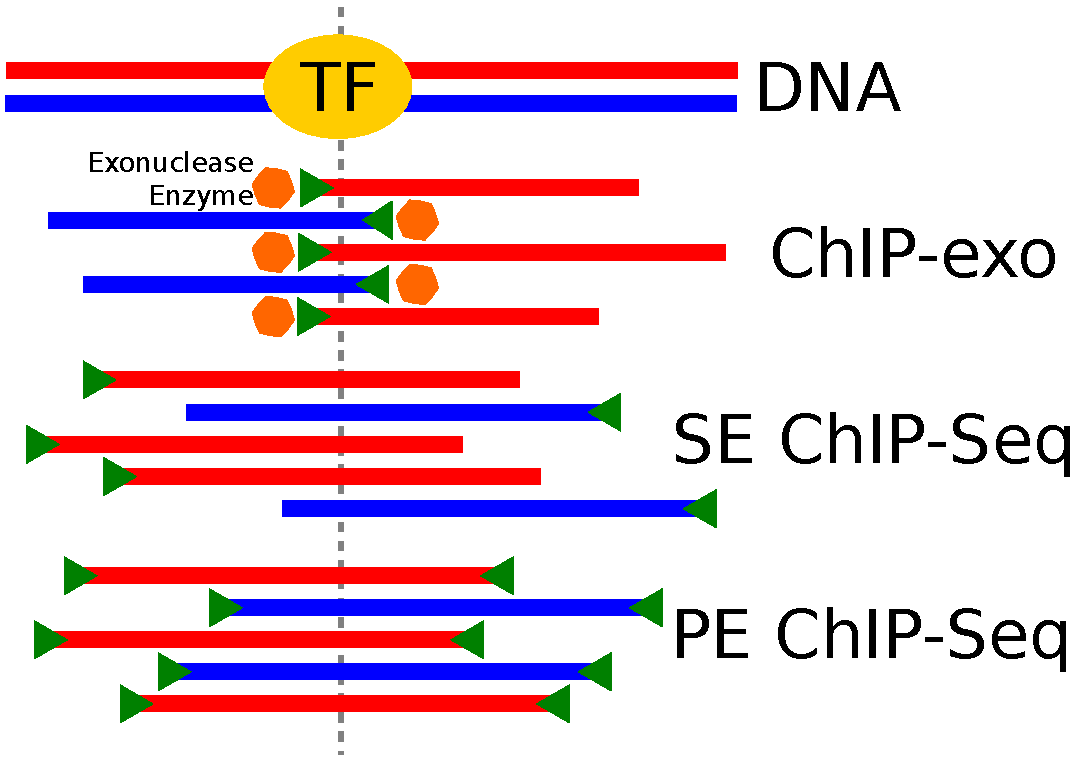
\includegraphics[width =
  .95 \textwidth]{/p/keles/ChIPexo/volume3/ChIPexo/figs/for_paper/chip_explanation_withEnzyme.pdf}
  % \caption{\textbf{Description of ChIP-exo, SE ChIP-Seq and PE
  %     ChIP-Seq:} A TF is bound to the forward (red) and backward
  %   (blue) strand of the DNA. Then, is sonicated: For ChIP-exo a
  %   exonuclease enzyme (orange hexagon) trims the $5\prime$ ends of
  %   each DNA fragment to a fixed distance from the bound protein,
  %   finally is subjected to Immunoprecipitation and amplification. For
  %   both ChIP-exo and SE ChIP-Seq an adapter is ligated (green
  %   triangles) at the $5\prime$ ends, while for PE ChIP-Seq is ligated
  %   to both ends.}
  \caption{A TF is bound to the forward (red) and backward (blue)
    strand of the DNA. Then, is sonicated: For ChIP-exo a exonuclease
    enzyme (orange hexagon) trims the $5\prime$ ends of each DNA
    fragment to a fixed distance from the bound protein, finally is
    subjected to Immunoprecipitation and amplification. For both
    ChIP-exo and SE ChIP-Seq an adapter is ligated (green triangles)
    at the $5\prime$ ends, while for PE ChIP-Seq is ligated to both
    ends.}
  \label{fig:chip_diagram}
\end{figure}
\newpage

\begin{figure}[h!]
\centering
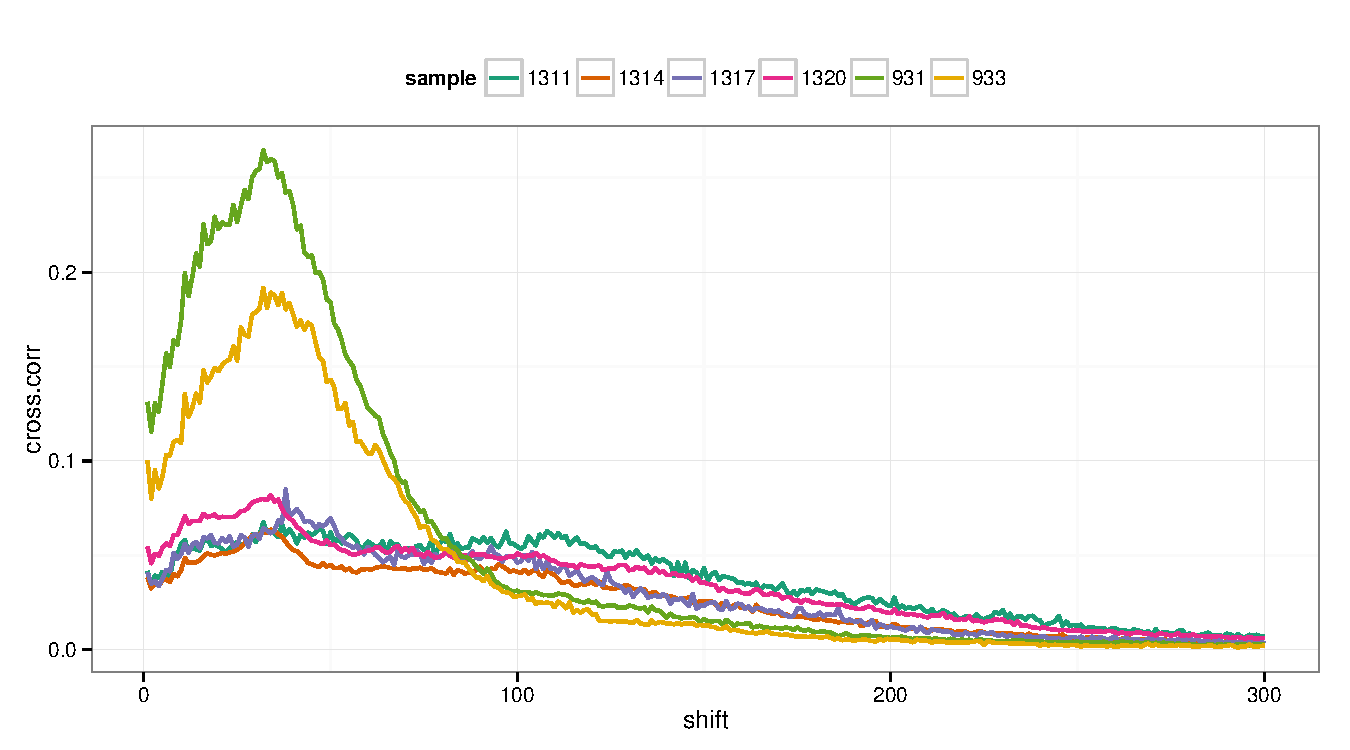
\includegraphics[width = .8\textwidth]{/p/keles/ChIPexo/volume3/ChIPexo/figs/for_paper/EColi_strand_cross_corr.pdf}
% \caption{\textbf{SCC curves for $\sig$ samples.} The ``phantom peak''
%   and the summit that corresponds to the read and fragment length
%   respectively are confounded due to the exonuclease digestion.}
\caption{SCC curves for $\sig$ samples. The ``phantom peak'' and the
  summit that corresponds to the read and fragment length respectively
  are confounded due to the exonuclease digestion.}
  \label{fig:scc_exo}
\end{figure}

\newpage

\begin{figure}[h!]
  \centering
  \includegraphics[width = .46\textwidth,page = 3 ]{../figs/for_paper/ChIPseqPET_ChIPexo_tagCount_comparison.pdf}
  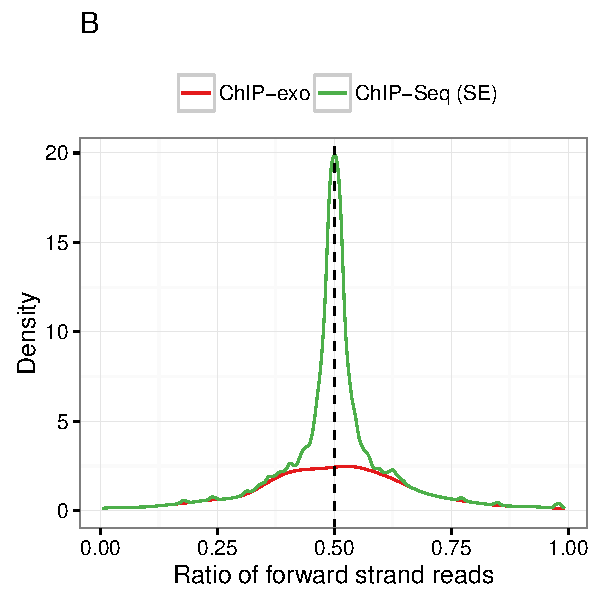
\includegraphics[width = .46\textwidth]{../figs/for_paper/forward_strand_ratio_comp_old.pdf}
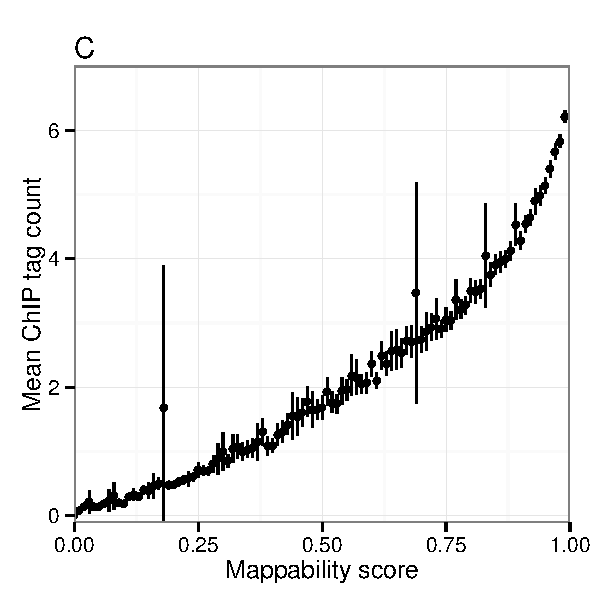
\includegraphics[width = .46\textwidth,page = 1]{../figs/for_paper/eukaryotic_bias_CTCF.pdf}
  \includegraphics[width = .46\textwidth,page = 2]{../figs/for_paper/eukaryotic_bias_CTCF.pdf}
  \caption{ A) Hexbin plot of PE ChIP-Seq bin counts vs ChIP-exo bin
    counts. B) Forward Strand Ratio densities for SE ChIP-Seq and
    ChIP-exo peaks. C) Mappability score vs mean ChIP tag counts with
    0.95 confidence bands. D) GC - content score vs mean ChIP tag
    counts with 0.95 confidence bands.}
  \label{fig:comp}
\end{figure}

% ChIP tag counts increase linearly as mappability scores
% increases. D) ChIP tag counts increase linearly as GC content score
% increases when GC content is less than 0.6 and then ChIP tag counts
% decrease as GC content increases. D) Percentage of sites with at
% least p.value.

\newpage

\begin{figure}[h!]
  \centering
  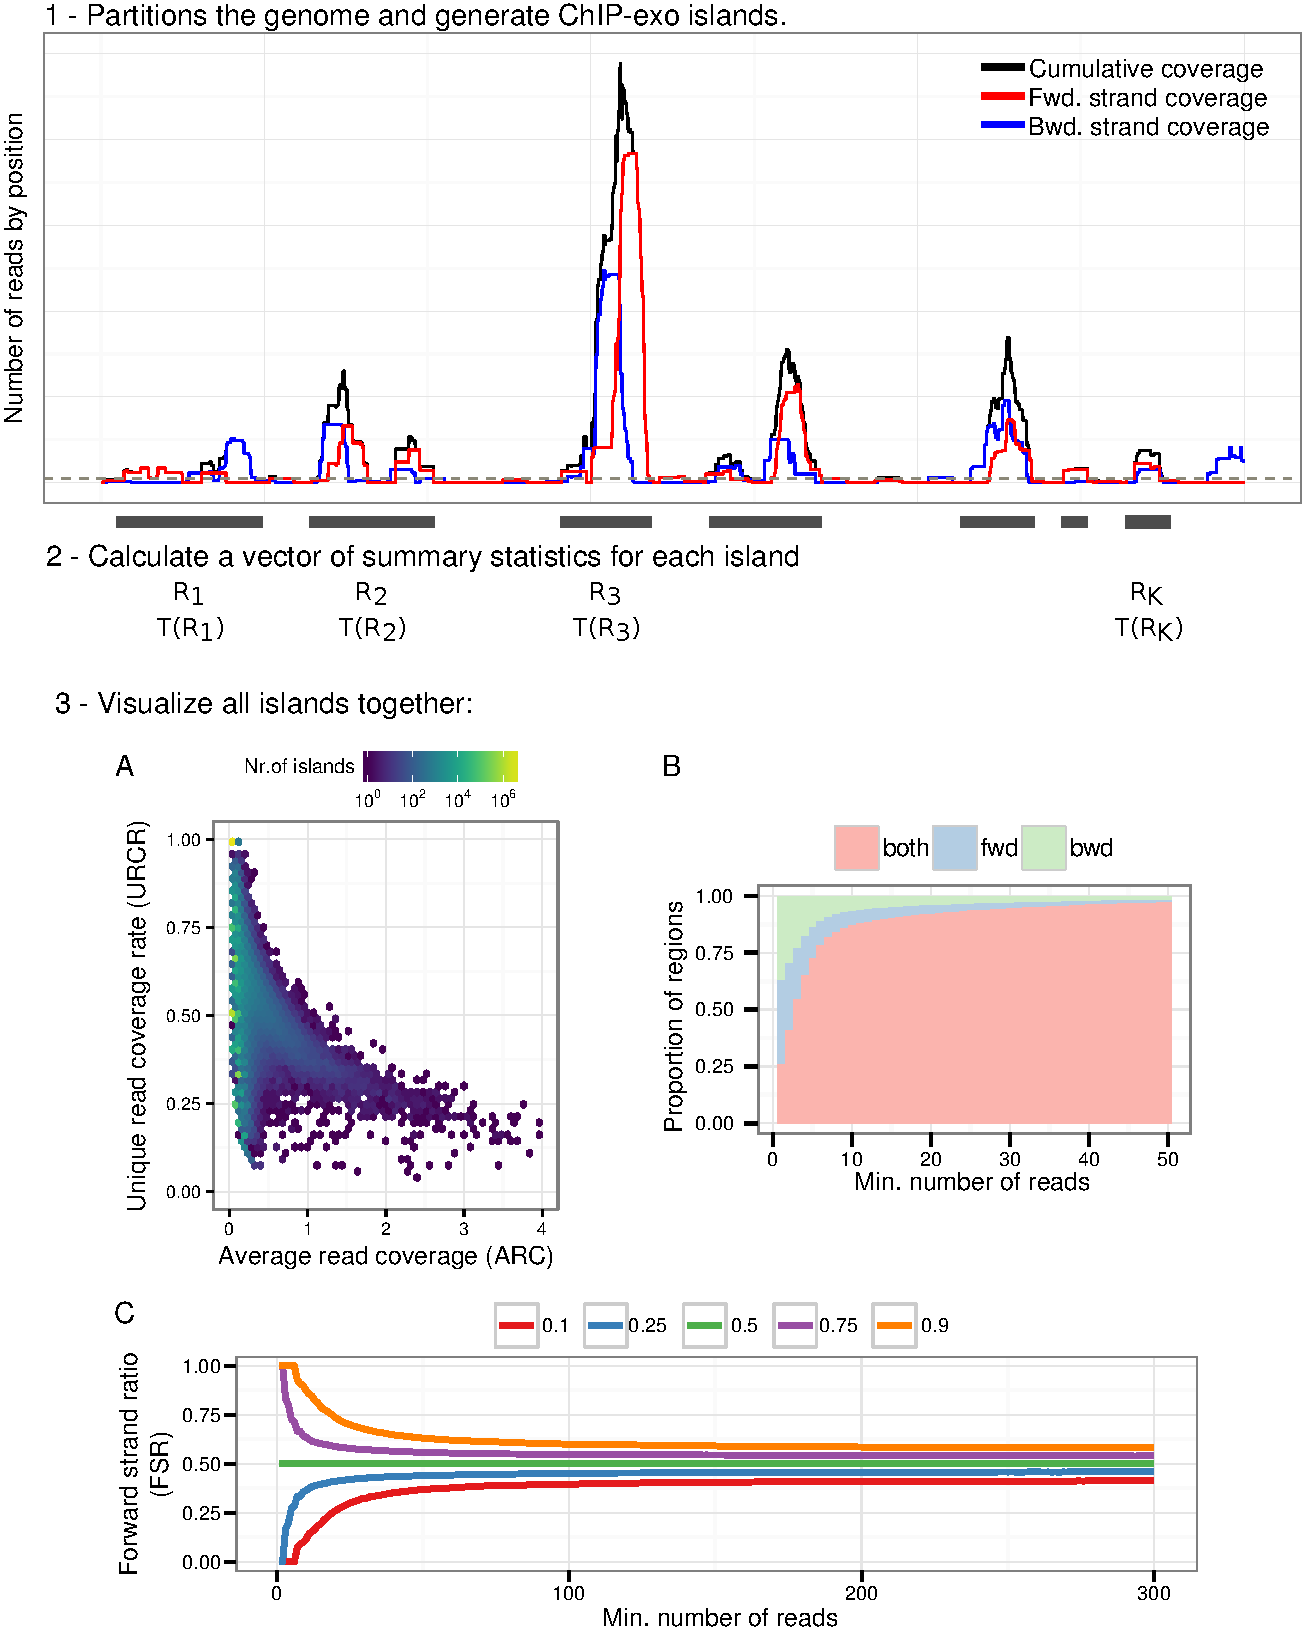
\includegraphics[width = \textwidth]{../figs/for_paper/coverage_diagram3.pdf}
  % \caption{\textbf{Flowchart of the ChIP-exo quality control
  %     pipeline.} A) ARC vs. URCR, this plot presents a global view of
  %   the balance between library complexity and enrichment. There are
  %   two arms: First, one with low ARC, which corresponds to regions
  %   formed by few aligned positions; Second, where the URCR decreases
  %   as the ARC increases. B) Min. depth vs Proportions of regions,
  %   this plot shows the strand composition for all the regions formed
  %   by a min. number of reads. Regions with low depth tend to be
  %   formed by undigested reads from one unique strand, while regions
  %   with higher signal are usually formed by reads in both strands. C)
  %   Min depth vs. FSR, this plot depicts how quickly the FSR's
  %   distribution approximate the median. In a high quality sample, the
  %   median is around 0.5, and the other quantiles reach that value
  %   quickly.}
  \caption{The ChIP-exo reads are partitioned by keeping the regions
    in the genome formed by the undigested fragments. For each region,
    we calculate a collection of summary statistics, which are
    visualized as A) ARC vs. URCR, this plot presents a global view of
    the balance between library complexity and enrichment. There are
    two arms: First, one with low ARC, which corresponds to regions
    formed by few aligned positions; Second, where the URCR decreases
    as the ARC increases. B) Min. depth vs Proportions of regions,
    this plot shows the strand composition for all the regions formed
    by a min. number of reads. Regions with low depth tend to be
    formed by undigested reads from one unique strand, while regions
    with higher signal are usually formed by reads in both strands. C)
    Min depth vs. FSR, this plot depicts how quickly the FSR's
    distribution approximate the median. In a high quality sample, the
    median is around 0.5, and the other quantiles reach that value
    quickly.}
  \label{fig:qcdiagram}
\end{figure}

\newpage

\begin{figure}[h!]
  \centering
  \includegraphics[width = .9  \textwidth,page = 1]{../figs/Carroll_mice_for_paper/FoxA1_enrichment.pdf}
  \newline
  \includegraphics[width = .3 \textwidth,page = 1]{../figs/FOXA1_mm9_fimo/FOXA1_summaries_by_replicate.pdf}
  \includegraphics[width = .3 \textwidth,page = 3]{../figs/FOXA1_mm9_fimo/FOXA1_summaries_by_replicate.pdf}
  \includegraphics[width = .3 \textwidth,page = 1]{../figs/FOXA1_mm9_fimo/FOXA1_log10pval_cumulative_nmotifs.pdf}
  \caption{Using the mouse FoxA1 experiment from \cite{exoillumina}:
    A) Hexbin plots of $\mbox{ARC}$ against $\mbox{URCR}$, there is a
    slight separation into two strong arms, one corresponds to low
    $\mbox{ARC}$ and varying $\mbox{URCR}$, and for the other
    $\mbox{URCR}$ decreases as $\mbox{ARC}$ increases. B) Number of
    candidate sites for each replicate. C) Percentage of candidate
    sites where the FoxA1 motif was detected. D) Cumulative
    proportion of detected motifs by replicate.}
  \label{fig:enrich}
\end{figure}

\newpage

\begin{figure}[h!]
  \centering  
  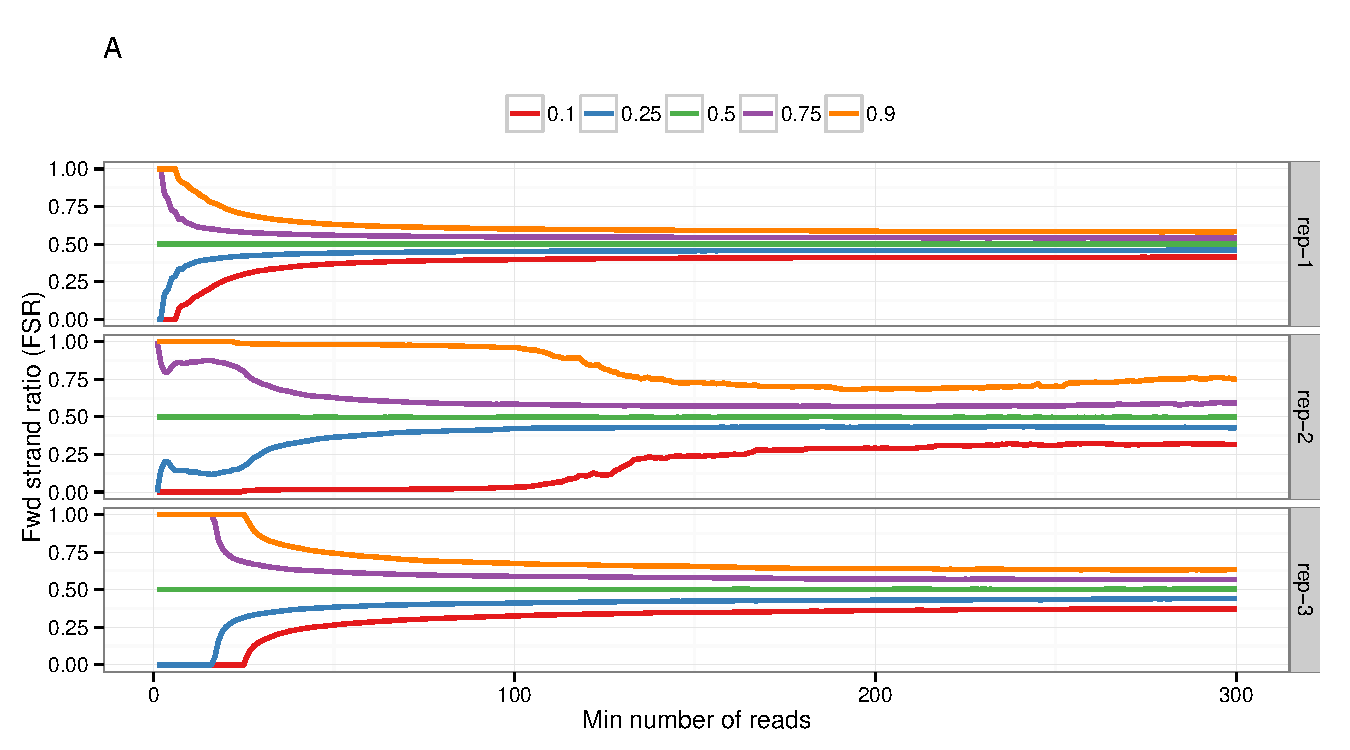
\includegraphics[width = .9\textwidth,page = 1]{../figs/Carroll_mice_for_paper/Strand_imbalance.pdf} 
  \newline
  \includegraphics[width = .9\textwidth,page = 2]{../figs/Carroll_mice_for_paper/Strand_imbalance.pdf} 
  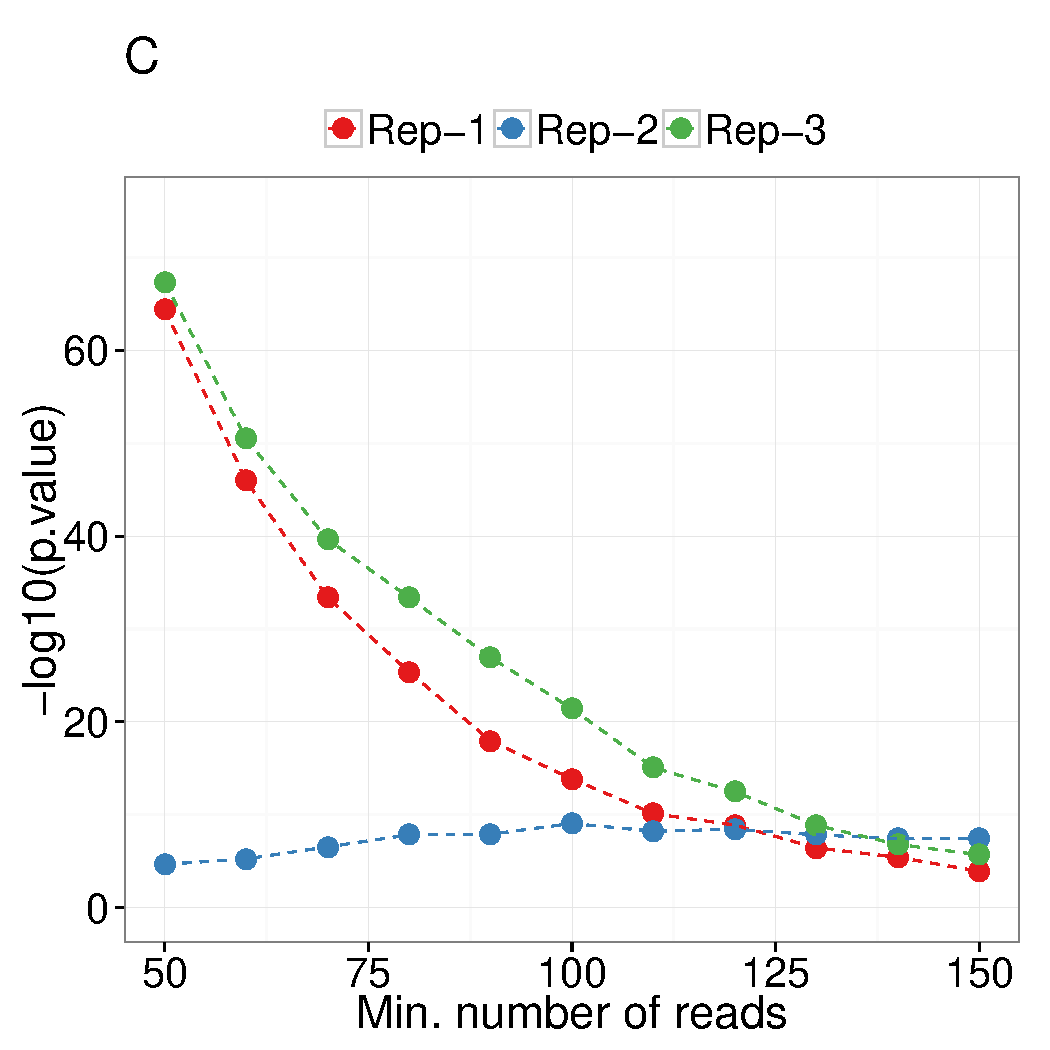
\includegraphics[width = .4\textwidth]{../figs/for_paper/Carroll_FSR_depth_VS_pvalWilcoxon.pdf}
  \caption{Strand imbalance QC plots for the same data as in Figure
    \ref{fig:enrich}A. A) FSR distribution quantiles as the lower
    depth regions are being filtered out, all quantiles approach to
    the median as the lower bound increases. B) Stacked histogram with
    the proportion of regions that are formed by two strands or only
    one, in a good sample the single-stranded regions are going to be
    filtered out quickly as in the middle row. C)
    $-\log_{10}(\text{p.value})$ of testing if the imbalance
    distributions differs when ChIP-exo regions overlap their peaks.}
  \label{fig:strand}
\end{figure}

\newpage

\begin{figure}[h!]
  \centering
  \includegraphics[width = .8\textwidth]{../figs/ChIPnexus/ChIPnexus_S2_MyC_enrichment.pdf}
\newline
  \includegraphics[width = .4\textwidth]{../figs/ChIPnexus/ChIPnexus_S2_MyC_fsr_surv.pdf}  
  \includegraphics[width = .4\textwidth]{../figs/ChIPnexus/ChIPnexus_S2_MyC_label_surv.pdf}  
  % \caption{\textbf{ChIP-exo QC pipeline on ChIP-nexus data.} A)
  %   Enrichment vs. library complexity, B) Strand imbalance and C)
  %   Single-strand region analysis for the MyC experiment in S2 cell
  %   lines in \emph{D. Melanogaster} from He et al., 2015
  %   \cite{chipnexus}}
  \caption{We applied the QC pipeline on ChIP-nexus data. A) ARC
    vs. URCR hexbin plots, B) FSR distribution quantiles and C)
    Stacked histogram with the proportion of regions composed by
    fragments on a single strand for the MyC experiment in S2 cell
    lines in \emph{D. Melanogaster} from He et al., 2015
    \cite{chipnexus}}
  \label{fig:nexus}
\end{figure}

\newpage


\begin{figure}[h!]
  \centering
  \includegraphics[width = .9  \textwidth,page = 1]{../figs/test_quantify/slope_npos_depth_boxplot.pdf}
  \includegraphics[width = .9  \textwidth,page = 1]{../figs/test_quantify/arc_urcr_param_regression.pdf}
  \includegraphics[width = .9  \textwidth,page = 2]{../figs/test_quantify/arc_urcr_param_regression.pdf}
  \caption{A) Comparison of change in depth as the number of unique
    position obtained by sampling 1,000 regions and fitting
    the model $\mbox{depth} = \beta \times \text{(\# unique
      positions)}$, and repeating this process 10,000 times. B)
    Intercept and C) Slope in the the $\mbox{URCR} = k / \mbox{ARC} +
    b$ model for the regions formed by more than 10 aligned
    positions.}
  \label{fig:enrich_all}
\end{figure}


\newpage
\begin{figure}[h!]
  \centering
  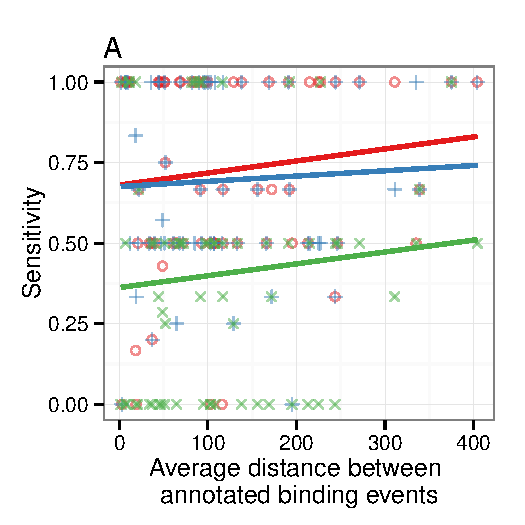
\includegraphics[width = .46\textwidth]{../figs/for_paper/sensitivity_exo_olda_data.pdf}
  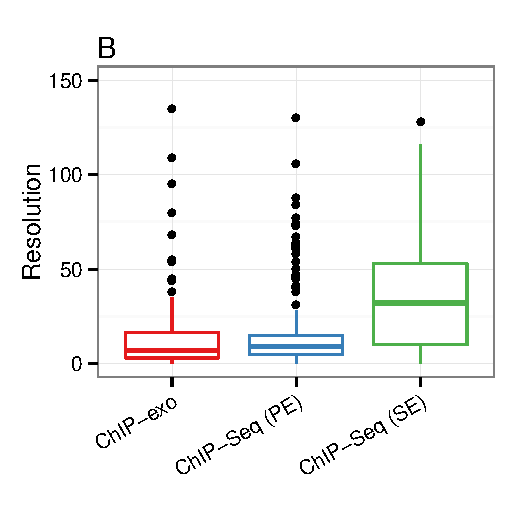
\includegraphics[width = .46\textwidth]{../figs/for_paper/resolution_by_dataset_old_data.pdf}
  \caption{Comparison of A) sensitivity and B) resolution between
    ChIP-exo and ChIP-Seq data. Sensitivity is defined as the
    proportion of RegulonDB annotations identified using each
    data. Resolution is defined as the distance between RegulonDB
    annotation and its closest prediction.}
  \label{fig:reso_all}
\end{figure}

\newpage

\begin{figure}[h]
  \centering
  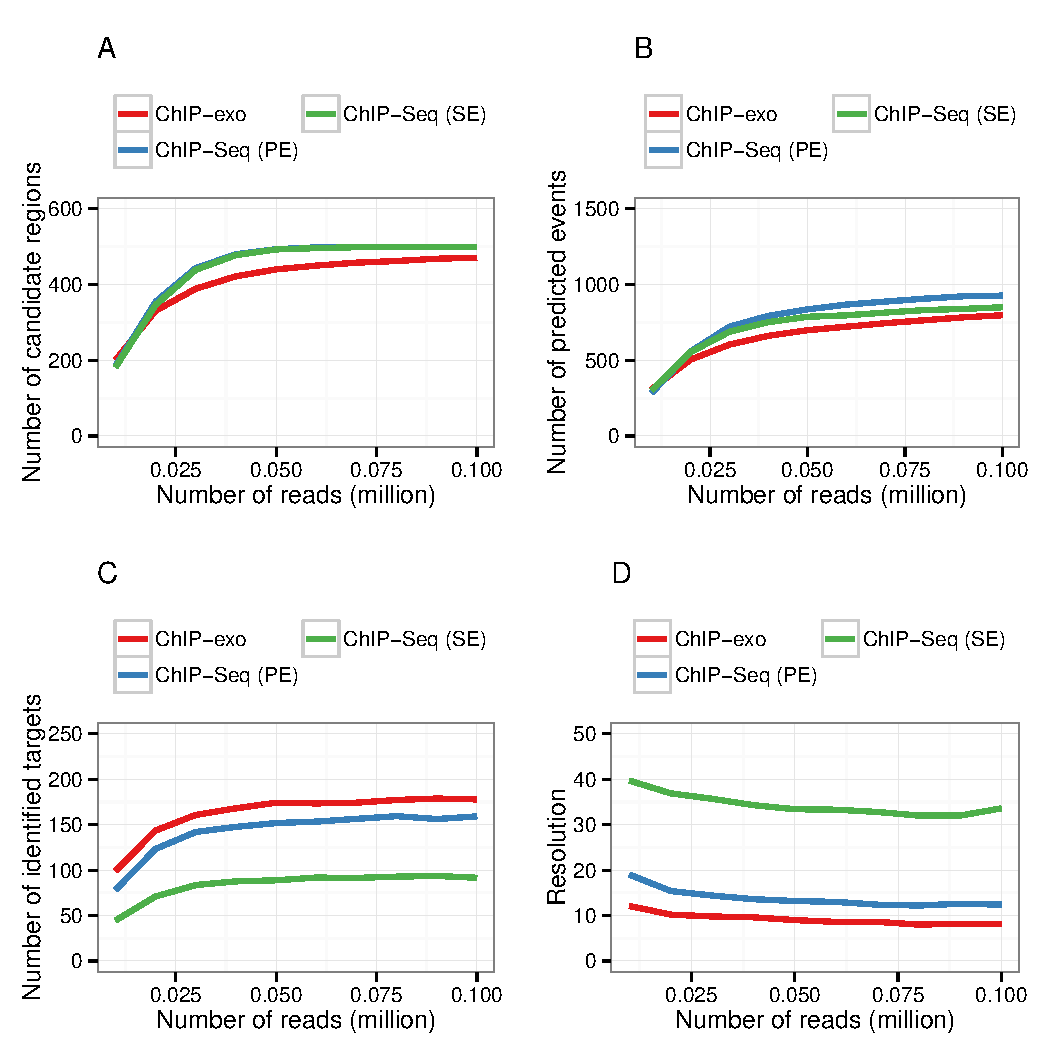
\includegraphics[width = .9\textwidth]{../figs/for_paper/saturation_analysis_old.pdf}
  \caption{Comparison of the number of A) candidate regions, B)
    predicted events, C) identified targets and D) resolution among
    ChIP-exo, PE ChIP-Seq and SE ChIP-Seq. RegulonDB annotations are
    considered as a gold standard. A gold standard binding events was
    deemed identified if a binding event was estimated at a $\pm$
    15 vicinity of it.}
  \label{fig:design}
\end{figure}


% \textbf{ChIP-exo, PE ChIP-Seq and SE ChIP-Seq comparison at varying
%   sequencing depths.} 
 \newpage

\begin{figure}[h!]
  \centering
\includegraphics[width = .9\textwidth]{../figs/saturation/K12_alignment/sig70_aerobic_enrichment.pdf}
\caption{Hexbin plots of ARC vs URCR of the $\sig$ ChIP-exo experiment
  under aerobic condition when 10K to 90K reads are being sampled.}
  \label{fig:exoQC_sat_aero}
\end{figure}

\newpage

\begin{figure}[h!]
  \centering
  \includegraphics[width = .9\textwidth]{../figs/for_paper/sig70_methods_comparison_FDR5_topM300.pdf}
  \caption{Comparison of the resolution between dPeak, Gem, Mace and
    Peakzilla methods. Resolution is defined as the minimum distance
    between a RegulonDB annotation and a predicted binding event.}
  \label{fig:methods_comp}
\end{figure}

\newpage

\beginsupplement

\section*{Supplement}
\label{sec:supp}


\emph{Note: I am not sure whether to include several figures on this supplement}

%% \begin{table}[h!]
%%  %% need to fix format
%%   \centering

% \caption{Usual ChIP-Seq QC metrics as in table \ref{tab:qc} but
%   applied to Landick's chipseq data of the rif experiment}
% \end{table}

\begin{figure}[h!]
  \centering % note change to stat_density(geom = "line")
   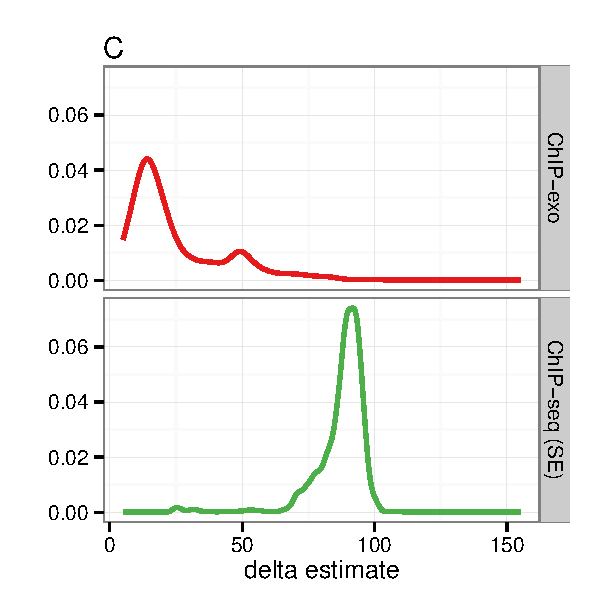
\includegraphics[width = .46\textwidth,page = 1]{../figs/for_paper/sigma_delta_old_densities.pdf}
   \includegraphics[width = .46\textwidth,page = 2]{../figs/for_paper/sigma_delta_old_densities.pdf}   
  \caption{ C) $\delta$ parameter in dPeak measures average distance
    of the reads to their respective binding site. In ChIP-exo data,
    reads were located much closer to the binding site than in SET
    ChIP-Seq. D) $\sigma$ parameter measure the dispersion of reads
    around each binding site. In ChIP-exo data, reads showed less
    variation around the their respective binding sites compared to
    SET ChIP-Seq.}

\end{figure}

\newpage

\begin{figure}[h!]
  \centering
  \includegraphics[width = .7\textwidth]{../figs/saturation/K12_alignment/PBC_saturation.pdf}
  \caption{Average PBC (among all seeds) of the sampled ChIP-exo, PE
    ChIP-Seq and SE ChIP-Seq experiments under the rif treatment
    conditions used for saturation analysis.}
  \label{fig:pbc_saturation}
\end{figure}

\newpage

\begin{figure}[h!] %%% fix this plot as one ggplot, facet_grid(condition ~ variable,scales = "free_y")
  \centering
  \begin{itemize}
  \item Rep-1 and rif-0min:
  \end{itemize}
  \includegraphics[width = .3\textwidth,page =2]{../figs/saturation/K12_alignment/Sig70_rep1_rif0_saturation_analysis.pdf}
  \includegraphics[width = .3\textwidth,page =3]{../figs/saturation/K12_alignment/Sig70_rep1_rif0_saturation_analysis.pdf}
  \includegraphics[width = .3\textwidth,page =4]{../figs/saturation/K12_alignment/Sig70_rep1_rif0_saturation_analysis.pdf}

  \begin{itemize}
  \item Rep-1 and rif-20min:
  \end{itemize}

  \includegraphics[width = .3\textwidth,page =2]{../figs/saturation/K12_alignment/Sig70_rep1_rif20_saturation_analysis.pdf}
  \includegraphics[width = .3\textwidth,page =3]{../figs/saturation/K12_alignment/Sig70_rep1_rif20_saturation_analysis.pdf}
  \includegraphics[width = .3\textwidth,page =4]{../figs/saturation/K12_alignment/Sig70_rep1_rif20_saturation_analysis.pdf}

  \begin{itemize}
  \item Rep-2 and rif-0min:
  \end{itemize}

  \includegraphics[width = .3\textwidth,page =2]{../figs/saturation/K12_alignment/Sig70_rep2_rif0_saturation_analysis.pdf}
  \includegraphics[width = .3\textwidth,page =3]{../figs/saturation/K12_alignment/Sig70_rep2_rif0_saturation_analysis.pdf}
  \includegraphics[width = .3\textwidth,page =4]{../figs/saturation/K12_alignment/Sig70_rep2_rif0_saturation_analysis.pdf}

  \begin{itemize}
  \item Rep-2 and rif-20min:
  \end{itemize}

  \includegraphics[width = .3\textwidth,page =2]{../figs/saturation/K12_alignment/Sig70_rep2_rif20_saturation_analysis.pdf}
  \includegraphics[width = .3\textwidth,page =3]{../figs/saturation/K12_alignment/Sig70_rep2_rif20_saturation_analysis.pdf}
  \includegraphics[width = .3\textwidth,page =4]{../figs/saturation/K12_alignment/Sig70_rep2_rif20_saturation_analysis.pdf}
  \caption{Comparison of the number of predicted events (left),
    identified targets (middle) and resolution (right) among ChIP-exo,
    PE ChIP-Seq and SE ChIP-Seq. RegulonDB annotations are considered
    as gold standard. A RegulonDB binding events was deemed identified
    if a binding event was estimated at a $\pm$ 15 vicinity
    of it.}
  \label{fig:saturation_rif}
\end{figure}

% \textbf{ChIP-exo, PE ChIP-Seq and SE ChIP-Seq comparison at varying
%   sequencing depth} 

\newpage

\begin{figure}[h!]
  \centering
  \includegraphics[width = .9\textwidth,page = 1]{../figs/saturation/K12_alignment/sig70_rif_enrichment.pdf}
  \caption{ARC vs URCR hexbin plots of Rep-1 and rif-0min from $\sig$
    experiment when 100K to 900K reads are being sampled for each
    panel. }
  \label{fig:exoQC_sat1}
\end{figure}

\newpage

\begin{figure}[h!]
  \centering
  \includegraphics[width = .9\textwidth,page = 1]{../figs/saturation/K12_alignment/sig70_rif_enrichment.pdf}

  \caption{ARC vs URCR hexbin plots of Rep-1 and rif-20min from $\sig$ experiment when 100K to 900K reads are being
    sampled for each panel.}
  \label{fig:exoQC_sat2}
\end{figure}

\newpage

\begin{figure}[h!]
  \centering
  \includegraphics[width = .9\textwidth,page = 1]{../figs/saturation/K12_alignment/sig70_rif_enrichment.pdf}
  \caption{ARC vs URCR hexbin plots of Rep-2 and rif-0min from $\sig$
    experiment when 100K to 900K reads are being sampled for each
    panel.}
  \label{fig:exoQC_sat3}
\end{figure}

\newpage

\begin{figure}[h!]
  \centering
  \includegraphics[width = .9\textwidth,page = 1]{../figs/saturation/K12_alignment/sig70_rif_enrichment.pdf}
  \caption{ARC vs URCR hexbin plots of Rep-2 and rif-20min from $\sig$ experiment when 100K to 900K reads are being
    sampled for each panel.}
  \label{fig:exoQC_sat4}
\end{figure}


\end{document}


% LocalWords:  Ntimes
